%%=============================================================================
%% Proof Of Concept
%%=============================================================================
\chapter{Proof Of Concept}
\label{ch:poc}
Omdat Aucxis met een Microsoft georiënteerde werkwijze werkt, moet er aangetoond worden dat het mogelijk is om dit te realiseren op GCP. Voor deze Proof Of Concept (POC) wordt er een CI/CD pipeline geconfigureerd. Hierin wordt er een simpele .NET Core applicatie gecompileerd. Ook de meegeleverde testen worden uitgevoerd tijdens de compilatie. Hierna wordt de applicatie en de bijbehorende componenten gecomprimeerd en naar een lokale fileserver geüpload. De gecompileerde applicatie kan dan uitgebreid worden getest in een lokale test omgeving. Ook is er een stap voorzien in de pijpleiding om de gecompileerde applicatie tijdelijk op het Cloud platform te bewaren. Dit voor het geval er iets verkeerd loopt tijdens het testen of tijdens het uploaden.

De .Net applicatie is een simpele .Net core console applicatie. Het bestaat uit een klasse, \emph{MessageUtil~\ref{code:messageutil}}. Deze klasse bevat een variabele, twee constructors, een methode om de variabele op te vragen, een methode om de variabele te tonen met een toevoegsel en een hoofdmethode die uitvoerbaar is.

\lstset{
    language=C,
    breaklines=true,
    frame=single,
    commentstyle=\color{mygreen},
    keywordstyle=\color{blue},
    numberstyle=\tiny\color{mygray},
    stringstyle=\color{mymauve},
    captionpos=b,
    caption={C\# bestand MessageUtil.cs. Hoofd klasse van de applicatie \emph{MessageUtil}},
    label=code:messageutil
}
\begin{lstlisting}
using System;
using System.Threading;

namespace MessageUtil {
public class MessageUtilProgram {

private String p_message;

private MessageUtilProgram() { }
public MessageUtilProgram(String message) {
p_message = message;
}

public String Message {
get { return p_message; }
}
public String SaluteMessage(String m) {
Console.WriteLine("Hello\n{0}", m);
return "hello" + m;
}

static void Main(string[] args) {
MessageUtilProgram mup = new MessageUtilProgram("Aucxis");
Console.WriteLine("{0}", mup.Message);
//mup.SaluteMessage(mup.Message);
Thread.Sleep(60000);
}
}
}
\end{lstlisting}

Daarnaast is er ook een testklasse voorzien, \emph{MessageUtilTest~\ref{code:messageutiltest}}. Hierin staan er twee methodes. De eerste methode test de constructor die de variabele moet instellen. De tweede methode test een van de print methodes.

\lstset{
    language=C,
    caption={C\# Test klasse MessageUtilTest.cs, voor het testen van MessageUtil~\ref{code:messageutil}.},
    label=code:messageutiltest
}
\begin{lstlisting}
using Microsoft.VisualStudio.TestTools.UnitTesting;
using MessageUtil;

namespace MessageUtilTest {

[TestClass]
public class MessageUtilTests {

[TestMethod]
public void ConstructWorks() {
string testmessage = "Test";
MessageUtilProgram mup = new MessageUtilProgram(testmessage);

string value = mup.Message;
Assert.AreEqual(testmessage, value,"Message didn't set correctly");
}

[TestMethod]
public void SaluteWorks() {
string testmessage = "Test";
string expected = "helloTest";
MessageUtilProgram mup2 = new MessageUtilProgram(testmessage);

string value = mup2.SaluteMessage(mup2.Message);
Assert.AreEqual(expected, value, "Message didn't salute correctly");
}
}
}

\end{lstlisting}

De applicatie wordt in beide gevallen onveranderd gebruikt zodanig dat een potentieel verschil zichtbaar wordt. Dit is de basis waaruit vertrokken is voor de POC. Om de prijs en het aantal benodigde producten zo laag mogelijk te houden, is er in dit onderzoek gekozen om Git en GitHub te gebruiken als versiebeheersysteem. GitHub is volledig ondersteund door beide platformen. Ook voorzien beide Cloud platformen applicaties op GitHub om automatisch de gewenste repositories te verbinden aan de CI/CD pipeline.

Het uploaden van de gecomprimeerde applicatie wordt door middel van Secure File Transfer Protocol (SFTP) op een Linux Ubuntu machine gedaan. Deze maakt verbinding met een Docker container die lokaal op een Windows Server 2019 draait. Deze\emph{~\href{https://hub.docker.com/r/atmoz/sftp/}{Docker container}} deelt een directory met Windows zodanig dat dit volledig modulair is met andere besturingssystemen of situaties. SFTP werkt onderliggend op basis van Secure Shell (SSH). Om verbinding te maken is dus een wachtwoord nodig. Dit is een probleem aangezien de virtuele systemen in de Cloud niet interactief zijn. Dit is opgelost door het gebruik van\emph{~\href{https://linux.die.net/man/1/sshpass}{SSHPASS}}. Dit Linux pakket heeft de mogelijkheid om aan SSH-toepassingen het wachtwoord mede te geven. Weliswaar zonder encryptie van het wachtwoord. Hierdoor is het wachtwoord leesbaar. Er wordt enkel op deze wijze gewerkt om het geheel relatief simpel te houden. Voor productie omgevingen zou er met SSH-sleutels moeten worden gewerkt. De SFTP operatie op de Linux Ubuntu in de Cloud, wordt uitgevoerd door middel van het \emph{script~\ref{code:filetrans}}. Dit Bash script zorgt ervoor dat het SSHPASS pakket beschikbaar is en voert de SFTP transactie uit.

\lstset{
    language=bash,
    caption={Bash script filetrans.sh. Script installeert de juiste Linux packages en kopieert de bestanden met SFTP.},
    label=code:filetrans
}
\begin{lstlisting}
#! /bin/bash
apt-get update
apt-get -y upgrade
apt-get -y install sshpass
sshpass -p 'pwd' sftp -o StrictHostKeyChecking=accept-new -P 5151 -oBatchMode=no -b - TestU@server << !
cd documents
put /workspace/MessageUtil/bin/Release/netcoreapp3.1/win10-x64/messageutil-win10-x64.tar.gz
bye
!
\end{lstlisting}

De Cloud specifieke configuratie bestanden worden in de volgende secties verder verduidelijkt. Voor GCP in \emph{sectie~\ref{sec:VergelijkingGCP}} en voor het Azure DeVops platform \emph{sectie~\ref{sec:VergelijkingADV}}.

\subsection{Google Cloud Platform}
\label{sec:VergelijkingGCP}
Voor deze POC is er een nieuw project aangemaakt op Google Cloud. Als op Google Cloud een project verwijderd wordt, worden ook alle resources en aanrekeningen stopgezet. Ook omdat er dan per project producten en services toegewezen kunnen worden. Zo kan er optimaal voldaan worden aan de gebruiker zijn noden. Het nieuw gecreëerde project, heeft de naam ‘net-demo-project’ gekregen zoals in \emph{figuur~\ref{fig:GCP_POC_projn}}.

\begin{figure}[!htbp]
    \centering
    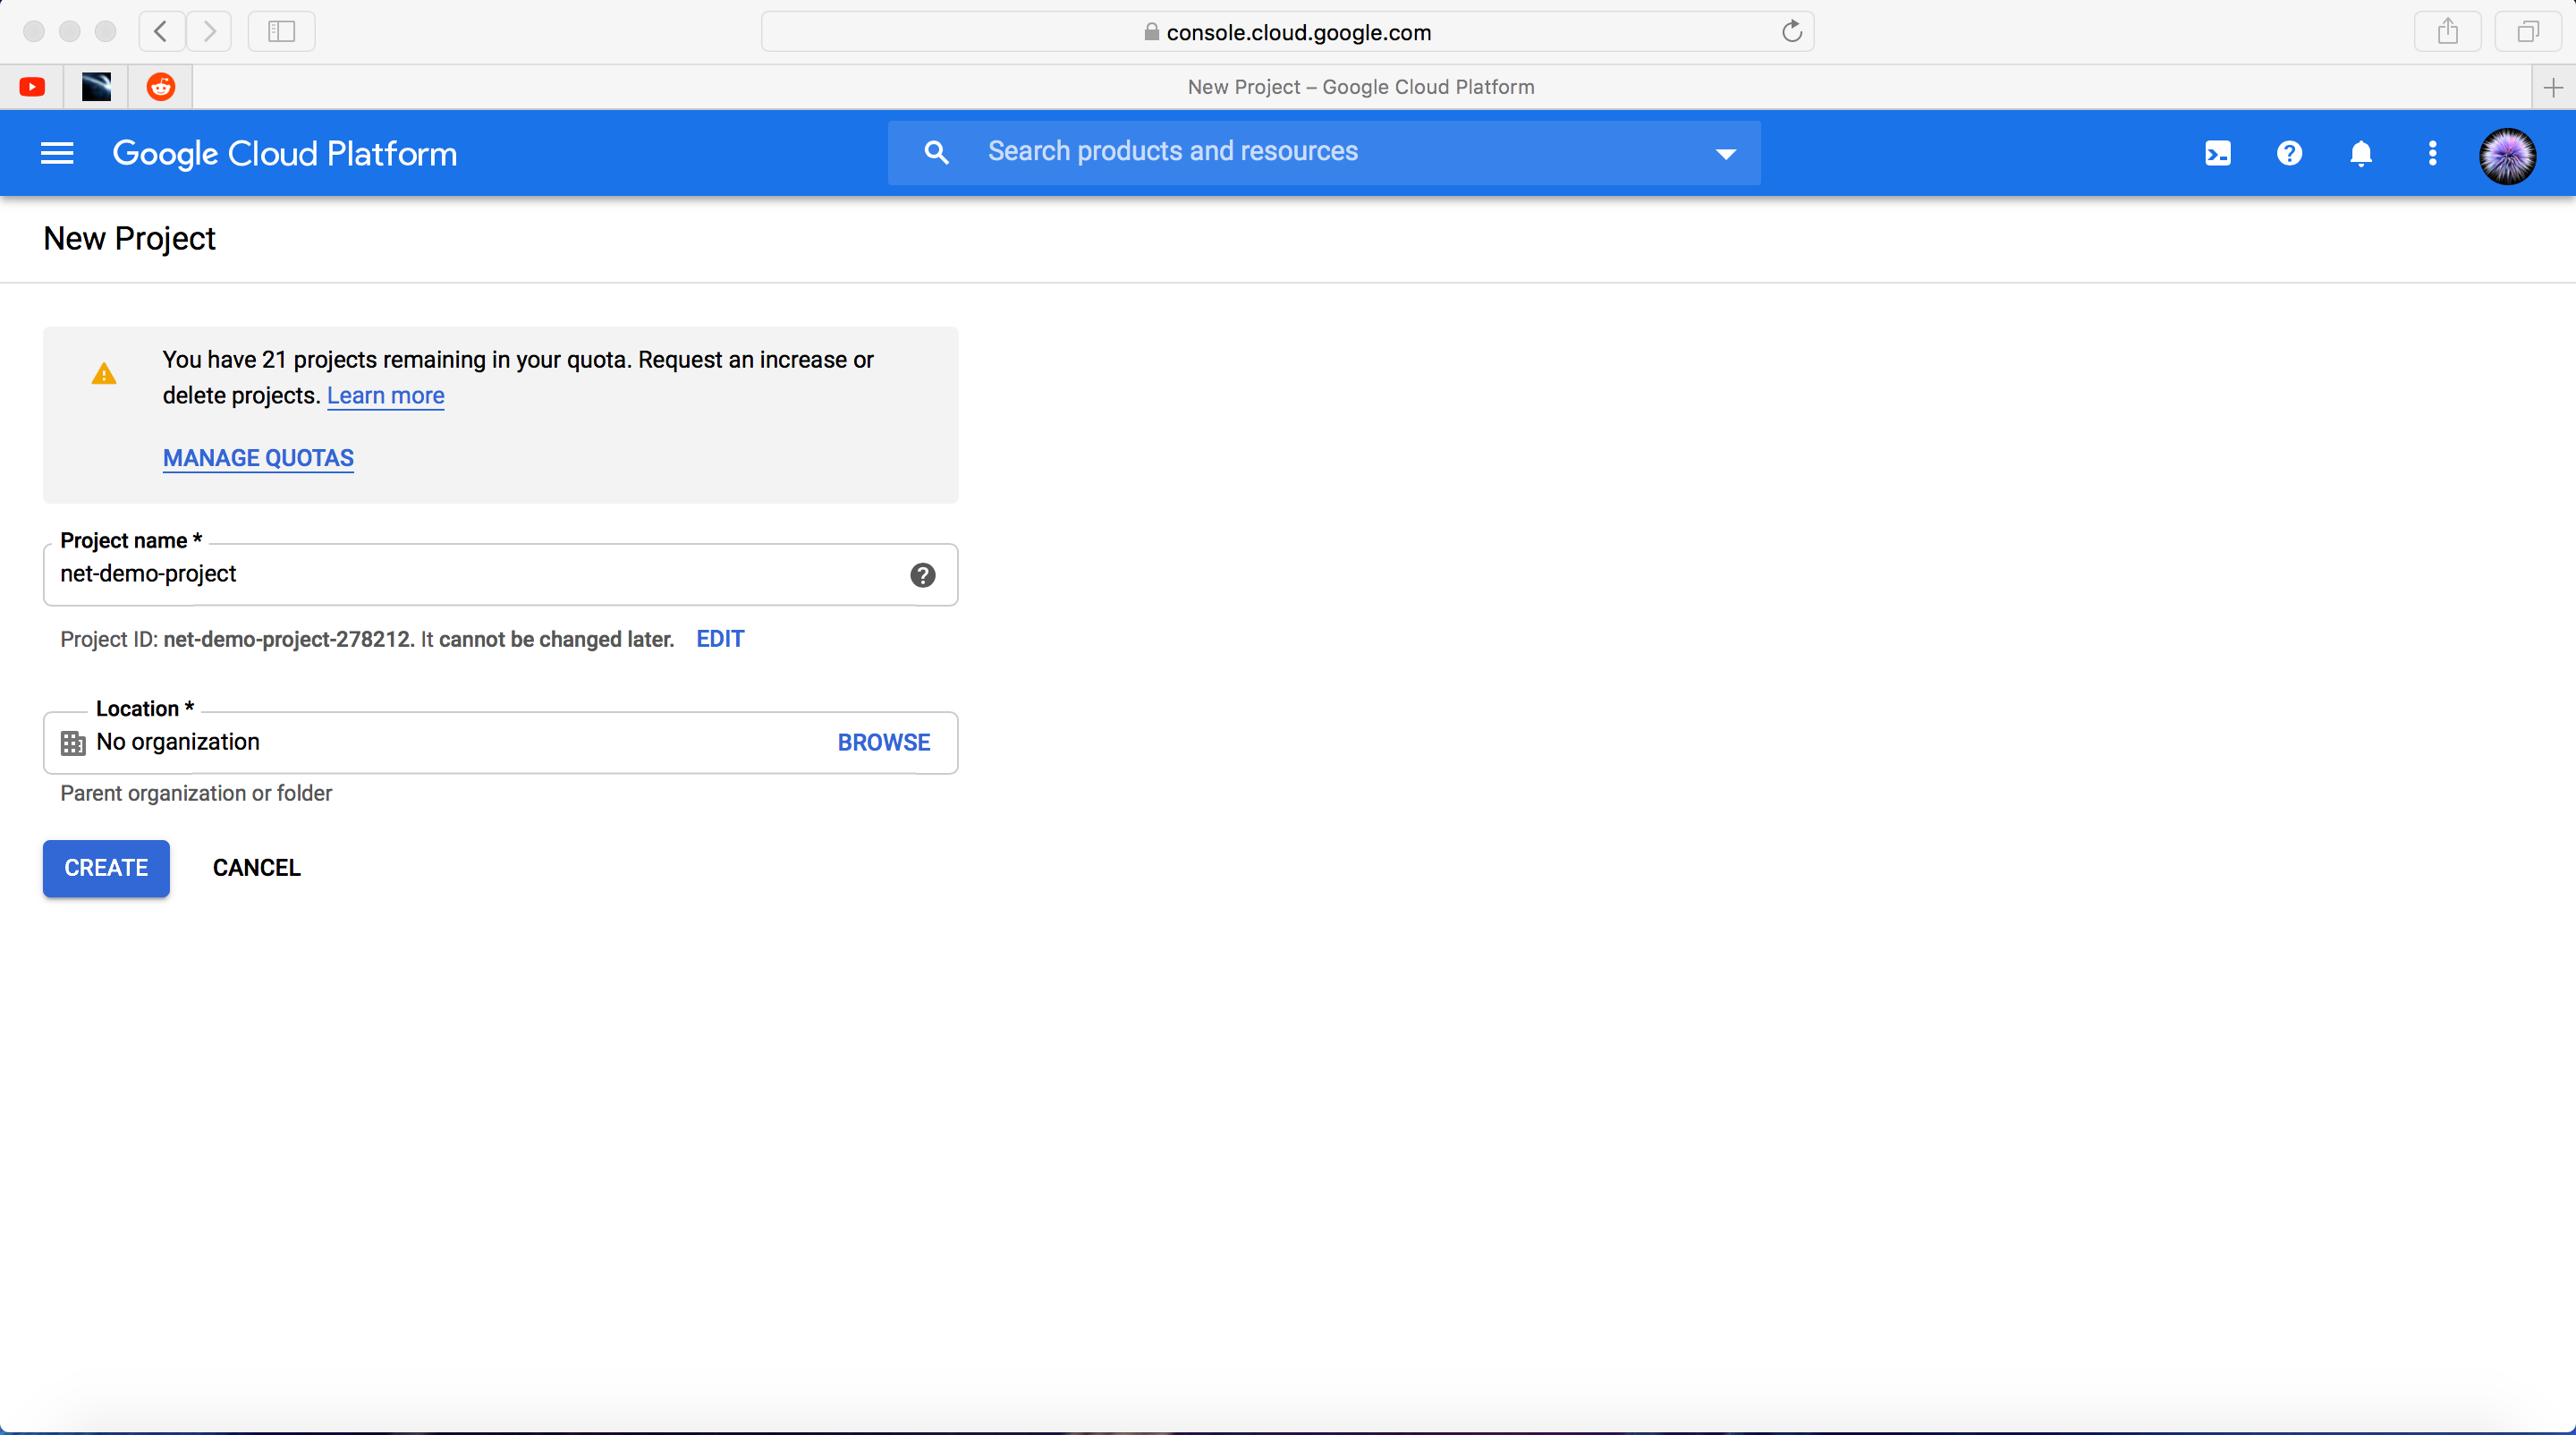
\includegraphics[width=\linewidth]{/Users/kenzie/Documents/HoGent/Bachelorproef/Images/gcp_net_demo_projn.png}
    \caption{New Project scherm op Google Cloud. Figuur toont het scherm om een nieuw project te creëren op Google Cloud.}
    \label{fig:GCP_POC_projn}
\end{figure}

Om Code Build op Google Cloud te gebruiken moest eerst de API via de online console worden geactiveerd. Ook moest er nog een Storage Bucket worden aangemaakt voor het opslaan van de gecompileerde applicatie. De Storage service is standaard geactiveerd en hoefde dus niet te worden aangezet. Deze Storage Bucket heeft de naam ‘net-demo-output-bucket’ gekregen. Ook belangrijk was de selectie voor de locatie van deze Storage Bucket. Hier is er gekozen voor een geografisch zo dicht mogelijke locatie. Dit om de overdracht tijden van bestanden zo minimaal mogelijk te houden. Alle andere opties zijn onveranderd gebleven. Ook is er de mogelijkheid om toegangsrechten toe te kennen. Dit kan interessant zijn voor een productie omgeving. \emph{Figuur~\ref{fig:GCP_POC_sb}}toont de gecreëerde Storage Bucket en de geselecteerde opties.

\begin{figure}[!htbp]
    \centering
    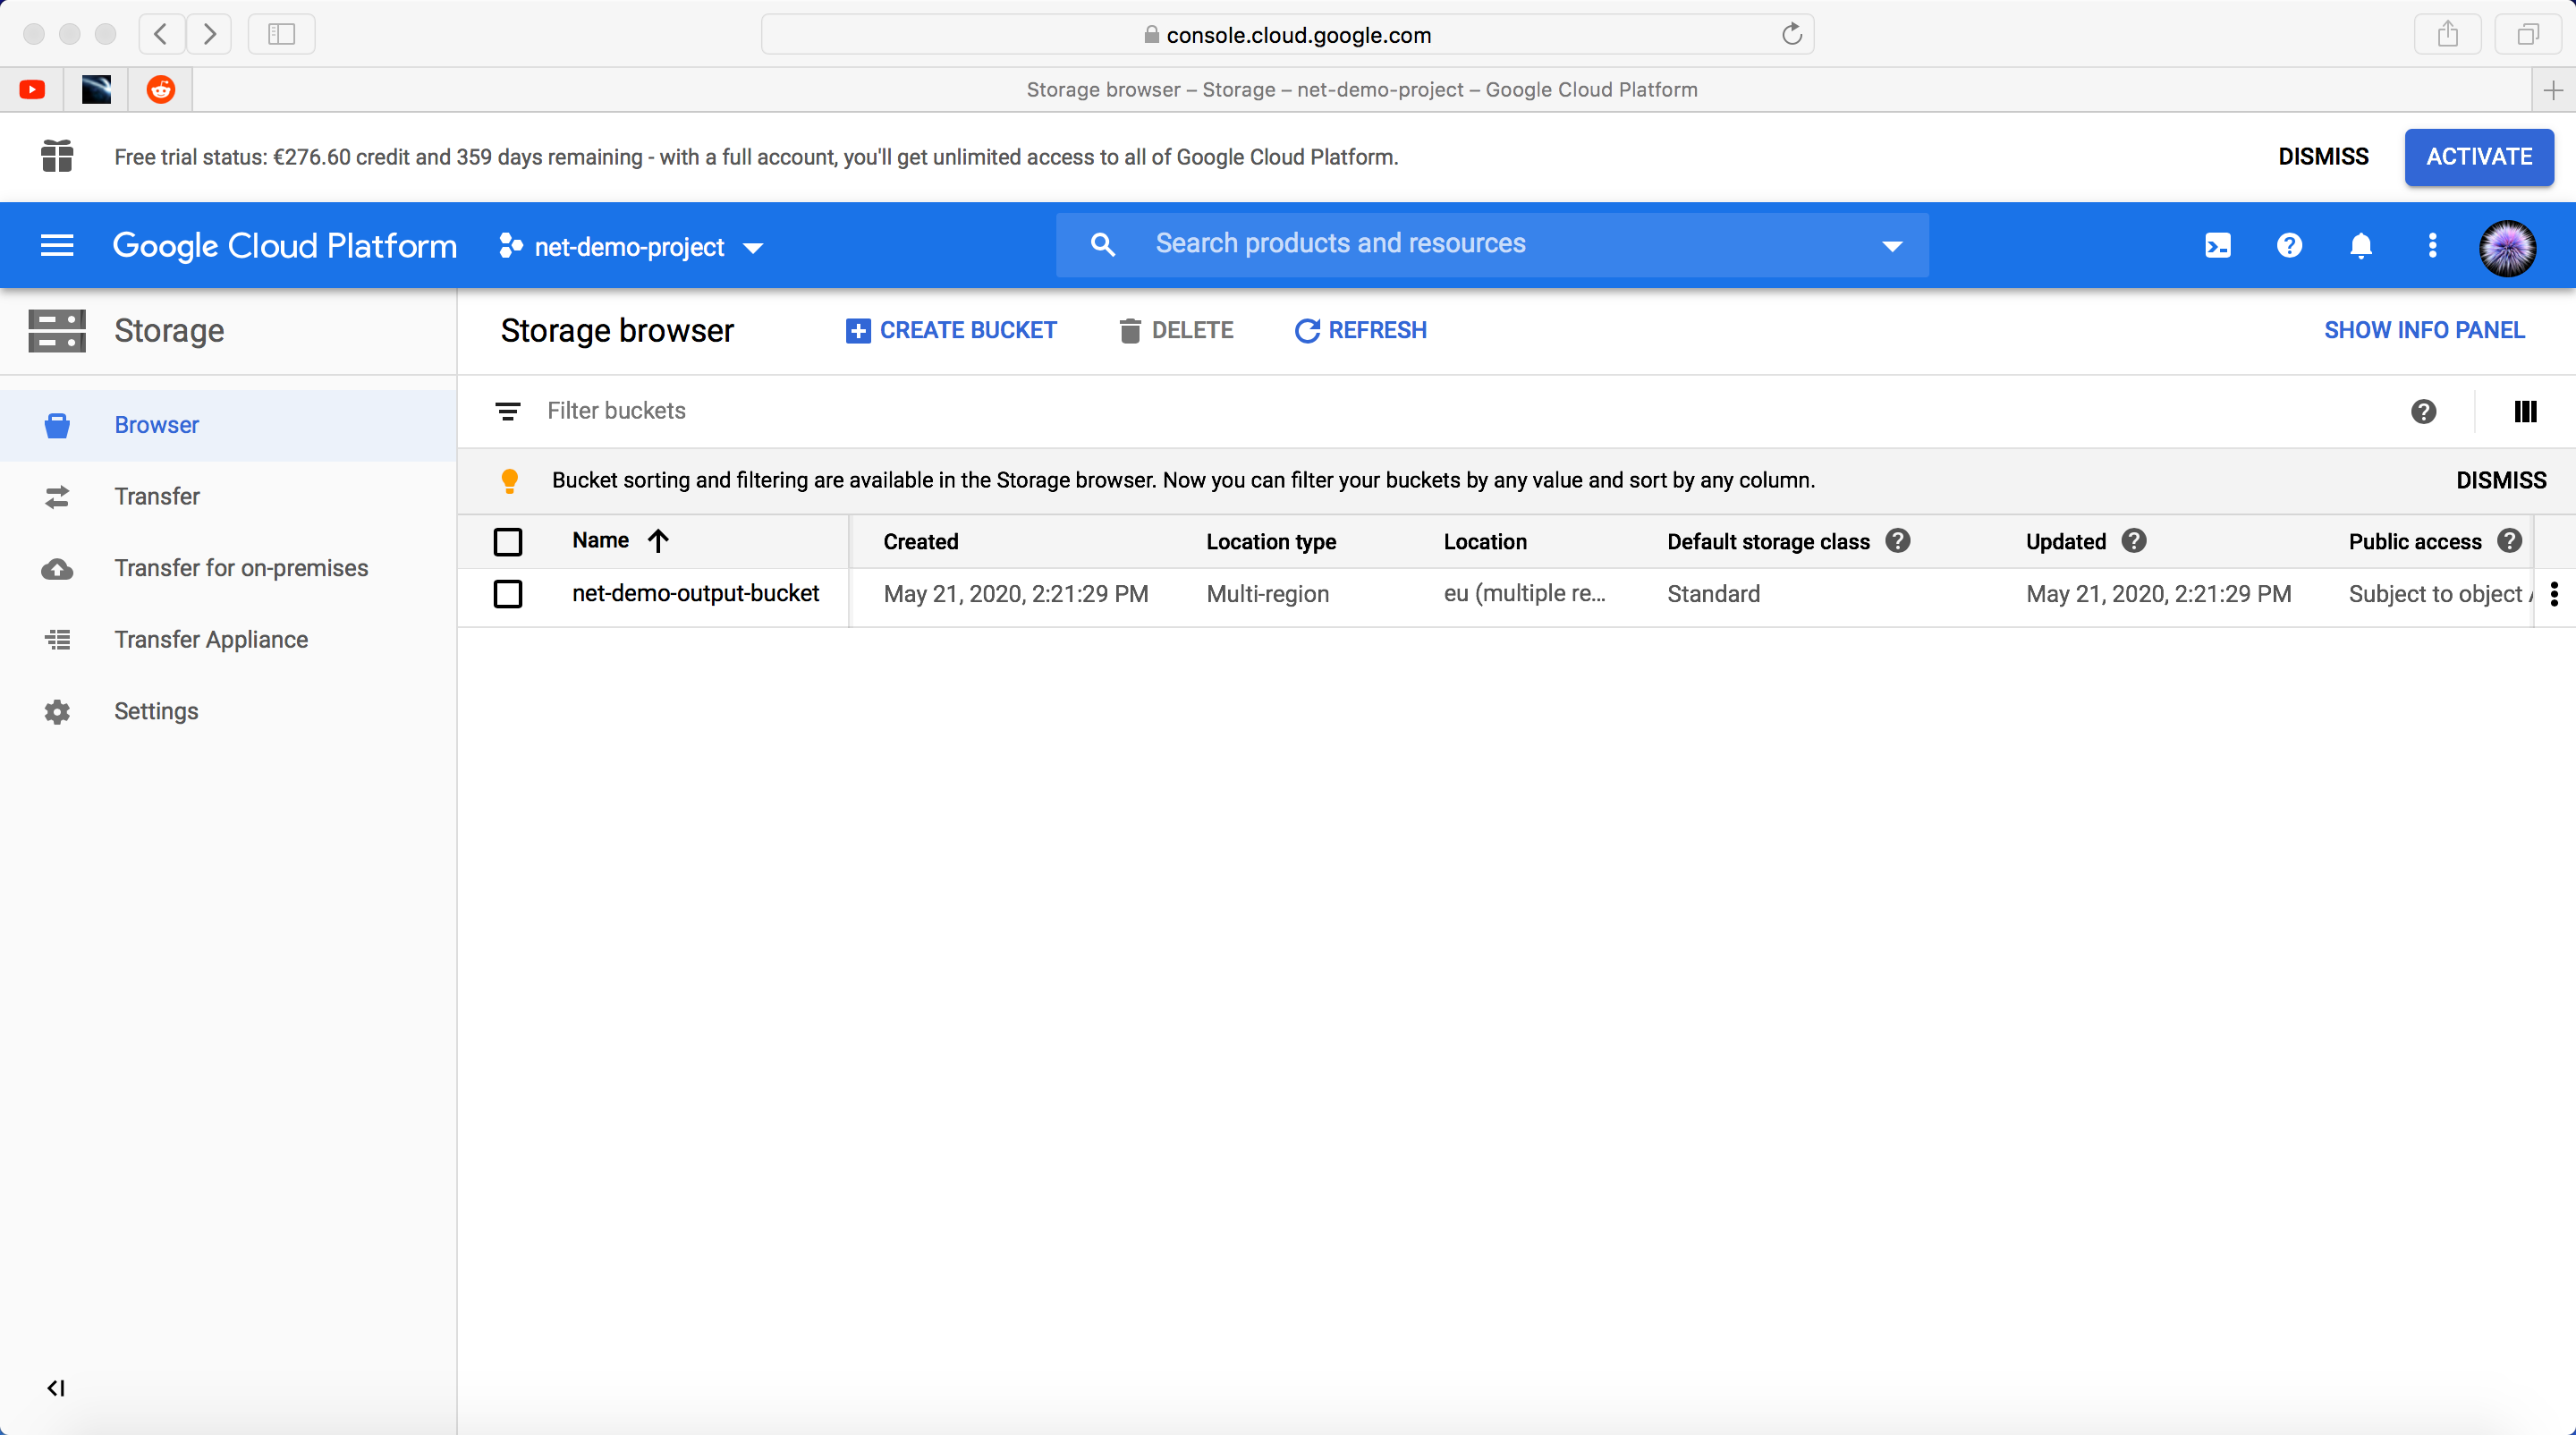
\includegraphics[width=\linewidth]{/Users/kenzie/Documents/HoGent/Bachelorproef/Images/gcp_net_demo_sb.png}
    \caption{Storage Bucket scherm op Google Cloud. Figuur toont het scherm met een gecreëerde Storage Bucket en de geconfigureerde opties op Google Cloud.}
    \label{fig:GCP_POC_sb}
\end{figure}

Hierna is er een nieuwe map aangemaakt op de gebruiker zijn computer voor de applicatie. Deze is geïnitialiseerd als een Git repository. Hierin zijn dan de bestanden, \emph{MessageUtil~\ref{code:messageutil}} \& \emph{MessageUtilTest~\ref{code:messageutiltest}} voor de .Net applicatie in geplaatst. Ook het \emph{script~\ref{code:filetrans}} voor de bestanden overdracht met SFTP is hierbij toegevoegd. Hiernaast is er ook een gitignore aangemaakt. \emph{Figuur~\ref{code:gcpgittree}} toont een tree van de bestanden en mappen structuur.

\lstset{
    language=bash,
    caption={Tree van de bestanden structuur voor de Proof Of Concept op Google Cloud.},
    label=code:gcpgittree
}
\begin{lstlisting}
poc_gcp_dotnet/
`--- .git
`--- .gitignore
`--- MessageUtil
`--- MessageUtil.csproj
`--- MessageUtilProgram.cs
`--- MessageUtil.sln
`--- MessageUtilTest
`--- MessageUtilTest.csproj
`--- MessageUtilTests.cs
`--- filetrans.sh
\end{lstlisting}

Vervolgens moest er connectie worden gemaakt met het gecreëerde project op Google Cloud met Google Cloud CLI. Hiervoor is op de CLI van de gebruiker zijn computer \emph{gcloud init -console only} uitgevoerd. Vervolgens is de wizard gevolgd en is het correcte project geselecteerd. Als volgende moest de configuratie van de CI/CD pipeline worden gemaakt. Zoals voorheen aangehaald werkt Google Cloud Code Build met Docker containers om al de gewenste taken uit te voeren. Voor deze POC is er gekozen om een Docker container van Microsoft zelf te gebruiken. Er is gekozen voor een .Net Core SDK container op \emph{\href{https://hub.docker.com/_/microsoft-dotnet-core-sdk}{DockerHub}}. Deze container wordt onderhouden door Microsoft zelf en heeft daarnaast ook uitgebreide documentatie ter beschikking op \emph{\href{https://github.com/dotnet/dotnet-docker/blob/master/samples/README.md}{GitHub}}. Zo moest er geen aangepaste container worden gemaakt die in de toekomst problemen zou kunnen krijgen naarmate de software update. Deze container is gebaseerd op een licht gewicht Linux machine. Hierop staat dan de SDK van Microsoft om .Net applicaties te testen, compileren, publiceren, enz.

Pipelines voor CI op Google Cloud Code Build worden geconfigureerd met behulp van een YAML-bestand. Voor deze POC zijn er vier verschillende stappen gedefinieerd met elk hun eigen doel. De eerste drie stappen maken allemaal gebruik van de door Microsoft gemaakte Docker container, ‘mcr.microsoft.com/dotnet/ore/sdk:3.1’. De laatste Docker container is een Ubuntu container. In de eerste stap worden de testen in \emph{MessageUtilTest~\ref{code:messageutiltest}} uitgevoerd. De tweede stap compileert de code van de applicatie specifiek voor een '64 Bit Windows 10' platform en maakt een folder publish aan. In een derde stap wordt het Bash script ‘tarring.sh’ uitgevoerd dat deze publish map comprimeert. \emph{Figuur~\ref{code:tarring}} toont dit Bash script. In een laatste stap wordt het 'filetrans' \emph{script~\ref{code:filetrans}} uitgevoerd. Ook is er een stukje code voorzien dat het gemaakte ‘artifact’ (de gecomprimeerde map) gaat uploaden naar een Storage Bucket op Google Cloud. \emph{Figuur~\ref{code:cloudbuildnet}} toont deze cloubuild.yaml. Google Cloud Code Build gaat automatisch bij de overgang van iedere stap naar een andere virtuele machine, het volume waarin wordt gewerkt monteren. Hierdoor zijn er geen speciale stappen of acties nodig om bestanden tussen de verschillende machines uit te wisselen.

\lstset{
    language=bash,
    caption={Bash script om een bepaalde folder te comprimeren tot een .tar.gz.},
    label=code:tarring
}
\begin{lstlisting}
#! /bin/bash
cd /workspace/MessageUtil/bin/Release/netcoreapp3.1/win10-x64/ && tar -zcvf messageutil-win10-x64.tar.gz ./publish/
\end{lstlisting}

\lstset{
    language=bash,
    caption={YAML-bestand voor de configuratie van de .Net pijpleiding op Google CLoud.},
    label=code:cloudbuilnet
}
\begin{lstlisting}
steps:
- name: 'mcr.microsoft.com/dotnet/core/sdk:3.1'
entrypoint: 'dotnet'
args: [ 'test' ]
- name: 'mcr.microsoft.com/dotnet/core/sdk:3.1'
entrypoint: 'dotnet'
args: [ 'publish', '-c', 'Release', '-r', 'win10-x64' ]
- name: 'mcr.microsoft.com/dotnet/core/sdk:3.1'
entrypoint: 'bash'
args: [ './tarring.sh' ]
- name: 'ubuntu'
entrypoint: 'bash'
args: [ './filetrans.sh']
artifacts:
objects:
location: 'gs://net-demo-output-bucket/'
paths: ['/workspace/MessageUtil/bin/Release/netcoreapp3.1/win10-x64/messageutil-win10-x64.tar.gz']
\end{lstlisting}

Nadat al deze bestanden zijn aangemaakt, is deze pijpleiding voor het eerst uitgevoerd. Hiervoor is de Google Cloud CLI gebruikt op de gebruiker zijn computer. Het commando\emph{gcloud builds submit} gaat de volledige Git repository kopiëren naar een tijdelijke Storage Bucket en start vervolgens de pijpleiding op volgens de configuratie vanuit 'cloudbuild.yaml'. Eenmaal dat deze pijpleiding volledig zonder fouten werkte, is de Git repository op GitHib geplaatst. Vervolgens is er via de online console op Google Cloud een Trigger aangemaakt om deze pijpleiding automatisch te laten uitvoeren bij het updaten van een bepaalde tak op GitHub. Hiervoor is GitHub gelinkt aan Google Cloud. \emph{Figuur~\ref{fig:GCP_POC_trigger}} toont de gemaakte Trigger en ook de specifieke tag die gebruikt is voor de tak op GitHub. Er is gekozen om deze Trigger op een specifieke tak van de GitHub repository te configureren om het aantal keren dat deze pijpleiding wordt uitgevoerd te kunnen minimaliseren. Zo kunnen de ontwikkelaars zelf kiezen wanneer ze de code willen compileren, door naar deze specifieke tak te uploaden. Dit vermijdt ook dat er in het wilde weg compilatie commando’s worden uitgevoerd door de ontwikkelaars zelf.

\begin{figure}[!htbp]
    \centering
    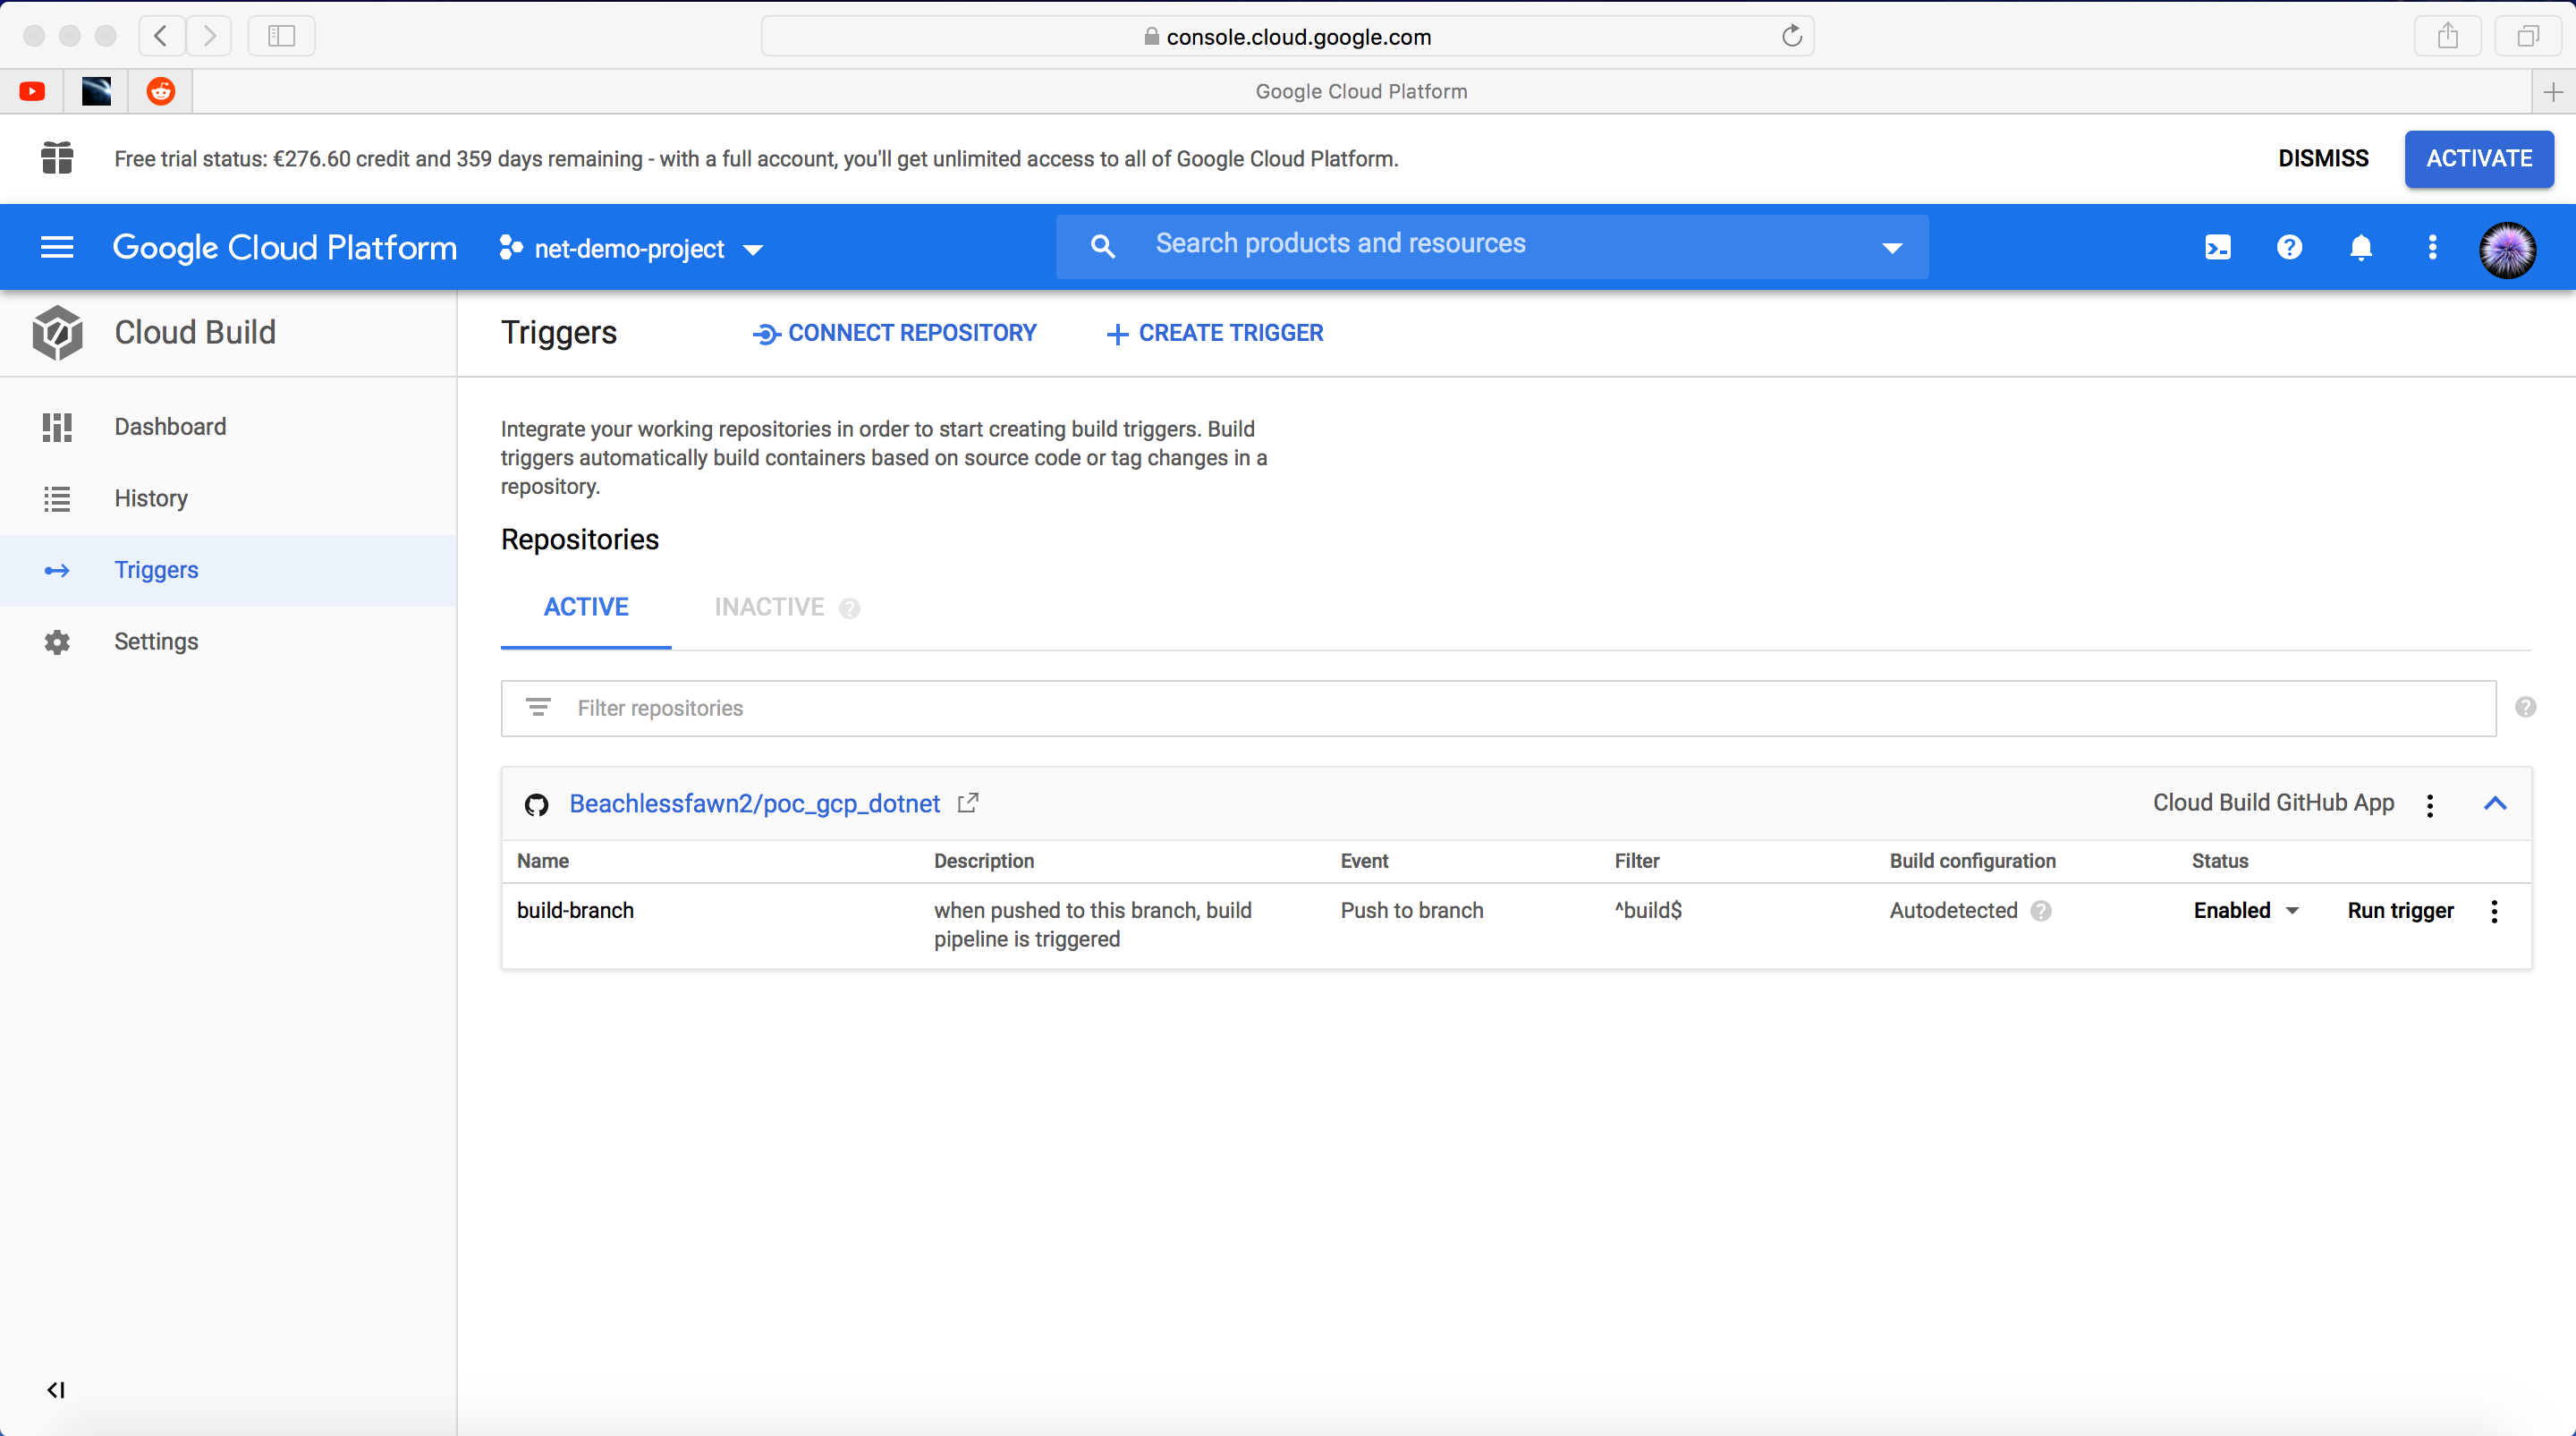
\includegraphics[width=\linewidth]{/Users/kenzie/Documents/HoGent/Bachelorproef/Images/gcp_net_demo_trigger.png}
    \caption{Scherm met Trigger voor een bepaalde pipeline op Google Cloud. Figuur toont het scherm  van Google Cloud met een gecreëerde Trigger op de tak 'Build' op GitHub.}
    \label{fig:GCP_POC_trigger}
\end{figure}

Eenmaal dit gebeurd is kon de trigger worden getest door een commit uit te voeren op GitHub. Vervolgens was het resultaat te testen op de lokale Windows Server 2019. Ook was er een gedetailleerd rapport te zien op de console van Google Cloud zelf. Om de applicatie uit te voeren moest simpel weg het gecomprimeerde bestand worden uitgepakt en uitgevoerd. \emph{Figuur~\ref{fig:GCP_POC_result}} toont het resultaat van de uitgevoerde applicatie op de lokale machine. \emph{Figuur~\ref{fig:GCP_POC_run}} toont de uitgevoerde compilatie op Google Cloud.

\begin{figure}[!htbp]
    \centering
    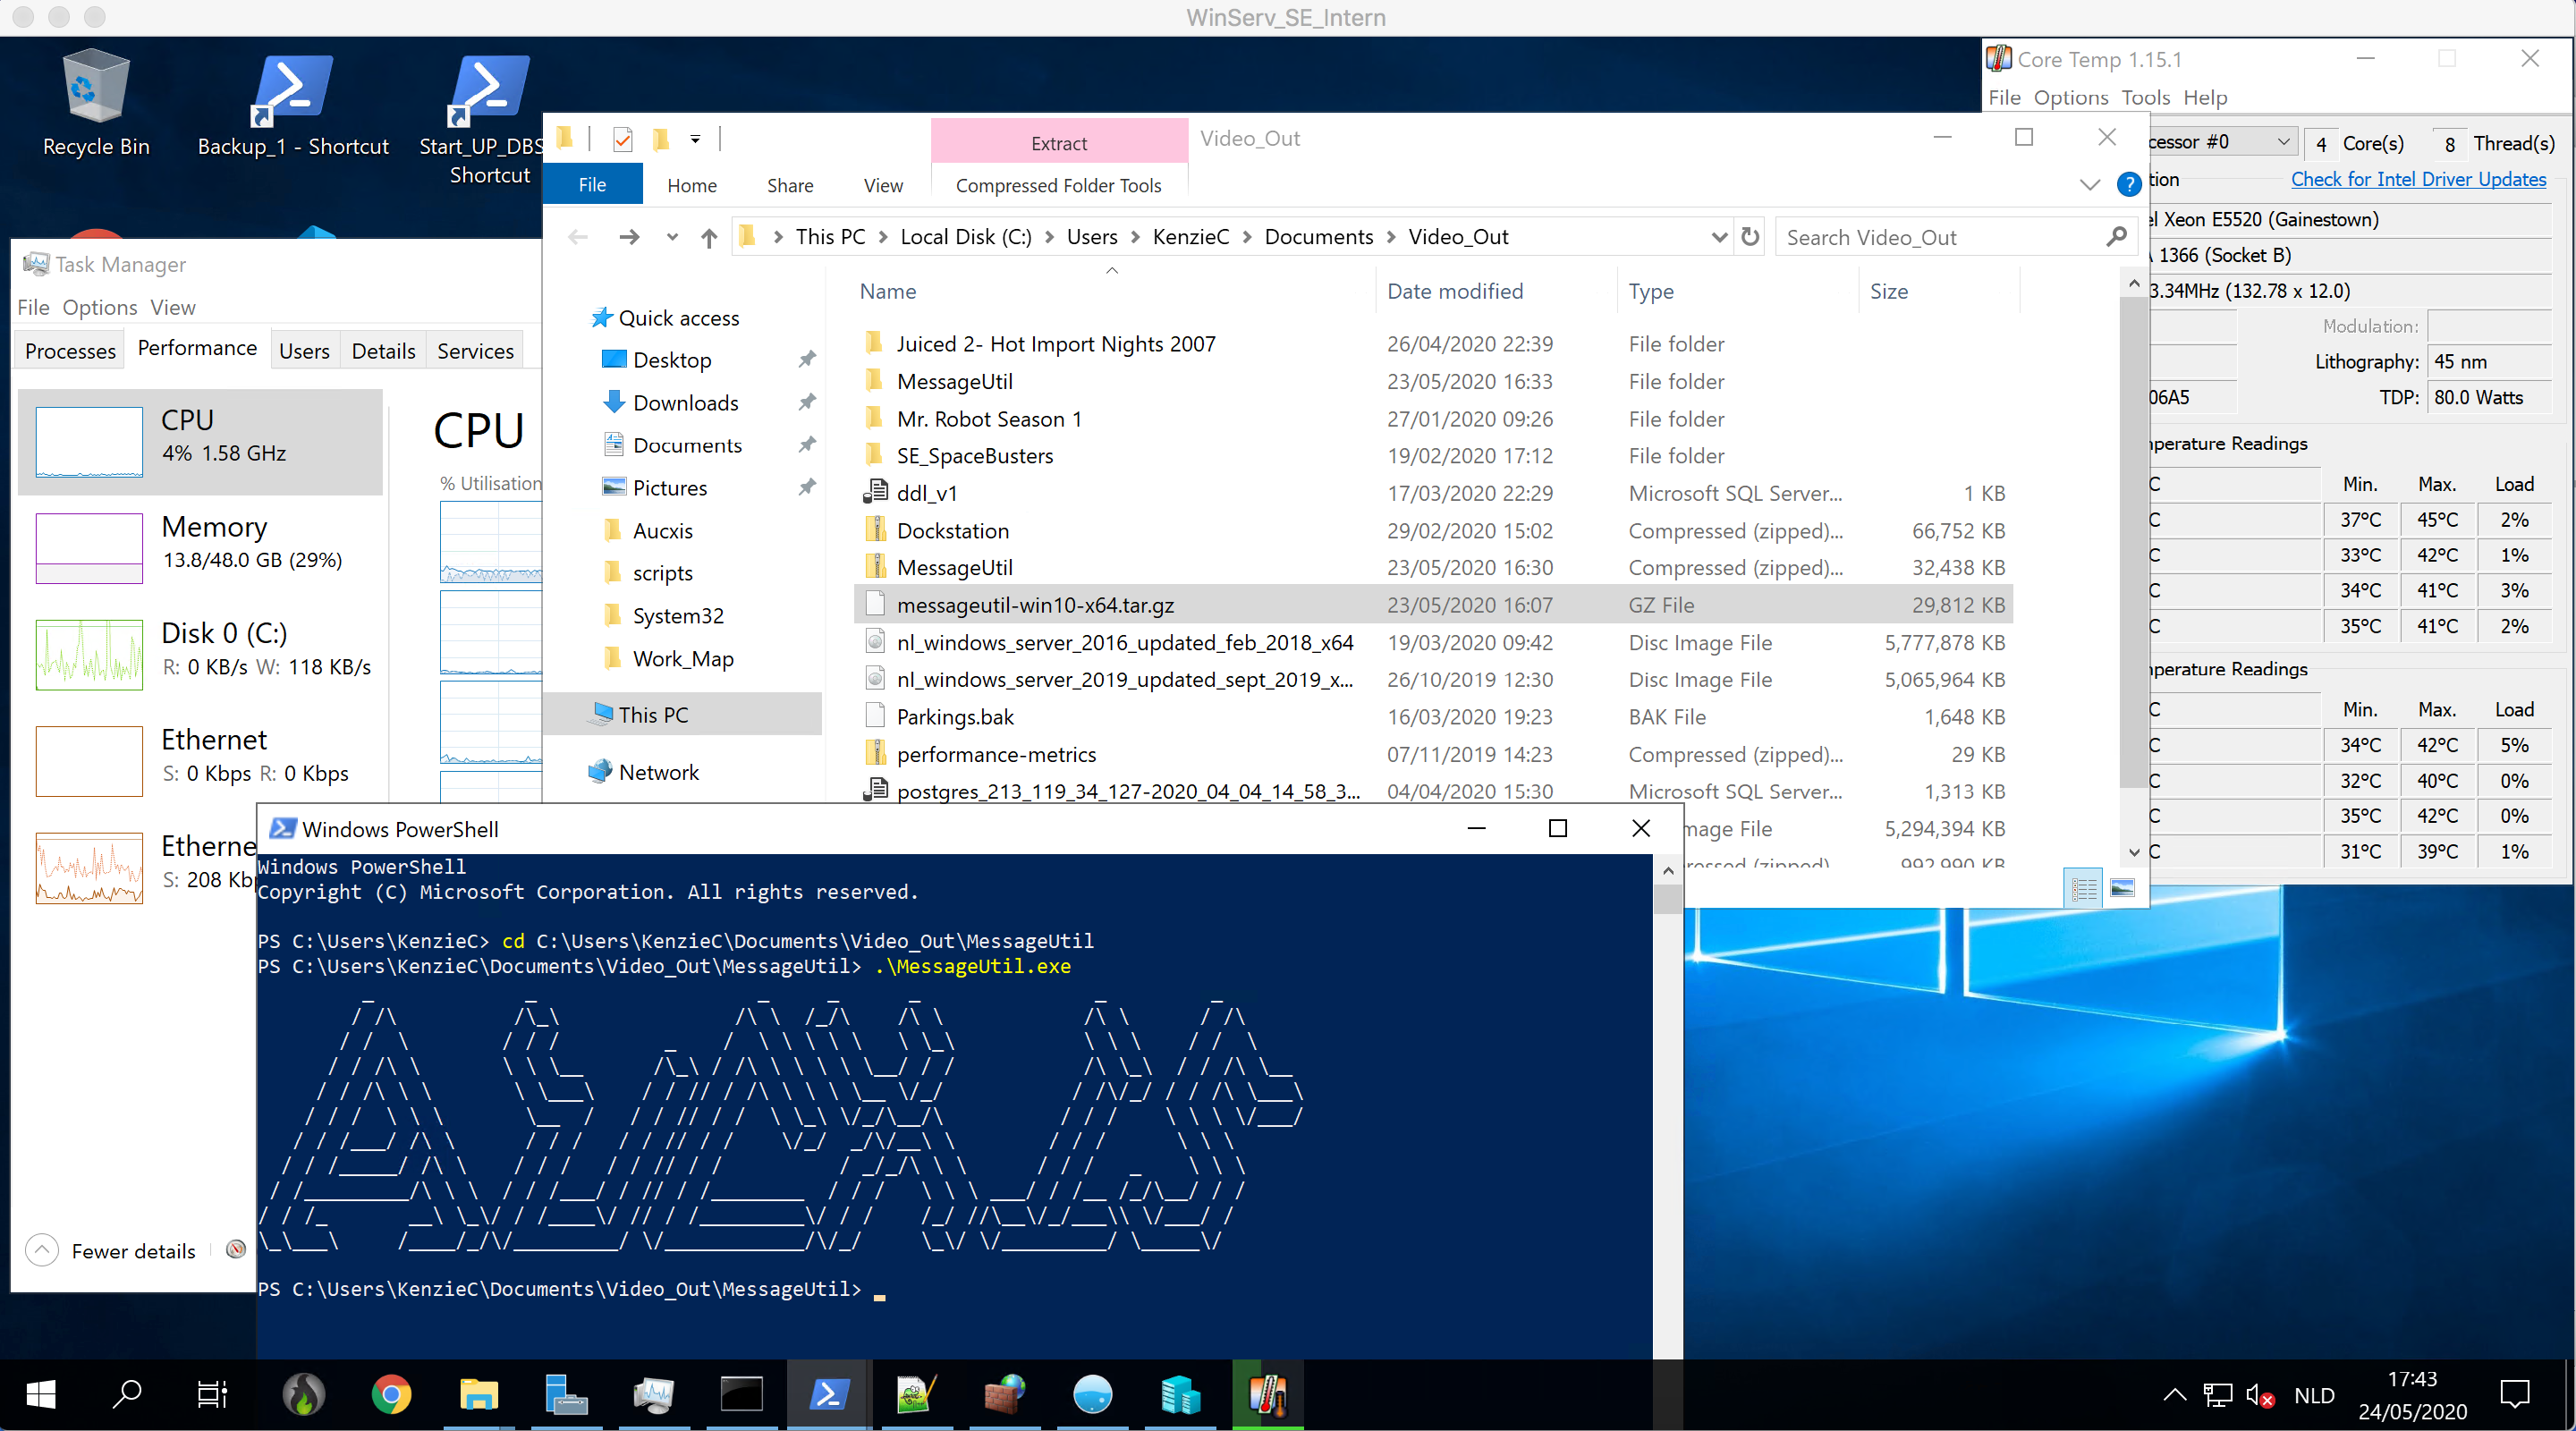
\includegraphics[width=\linewidth]{/Users/kenzie/Documents/HoGent/Bachelorproef/Images/gcp_net_demo_result.png}
    \caption{Resultaat ven de applicatie. Figuur toont de uitvoer van de gecompileerde applicatie op een lokale Windows Server 2019. Applicatie is gekopieerd door middel van \emph{script~\ref{code:filetrans}}.}
    \label{fig:GCP_POC_result}
\end{figure}

\begin{figure}[!htbp]
    \centering
    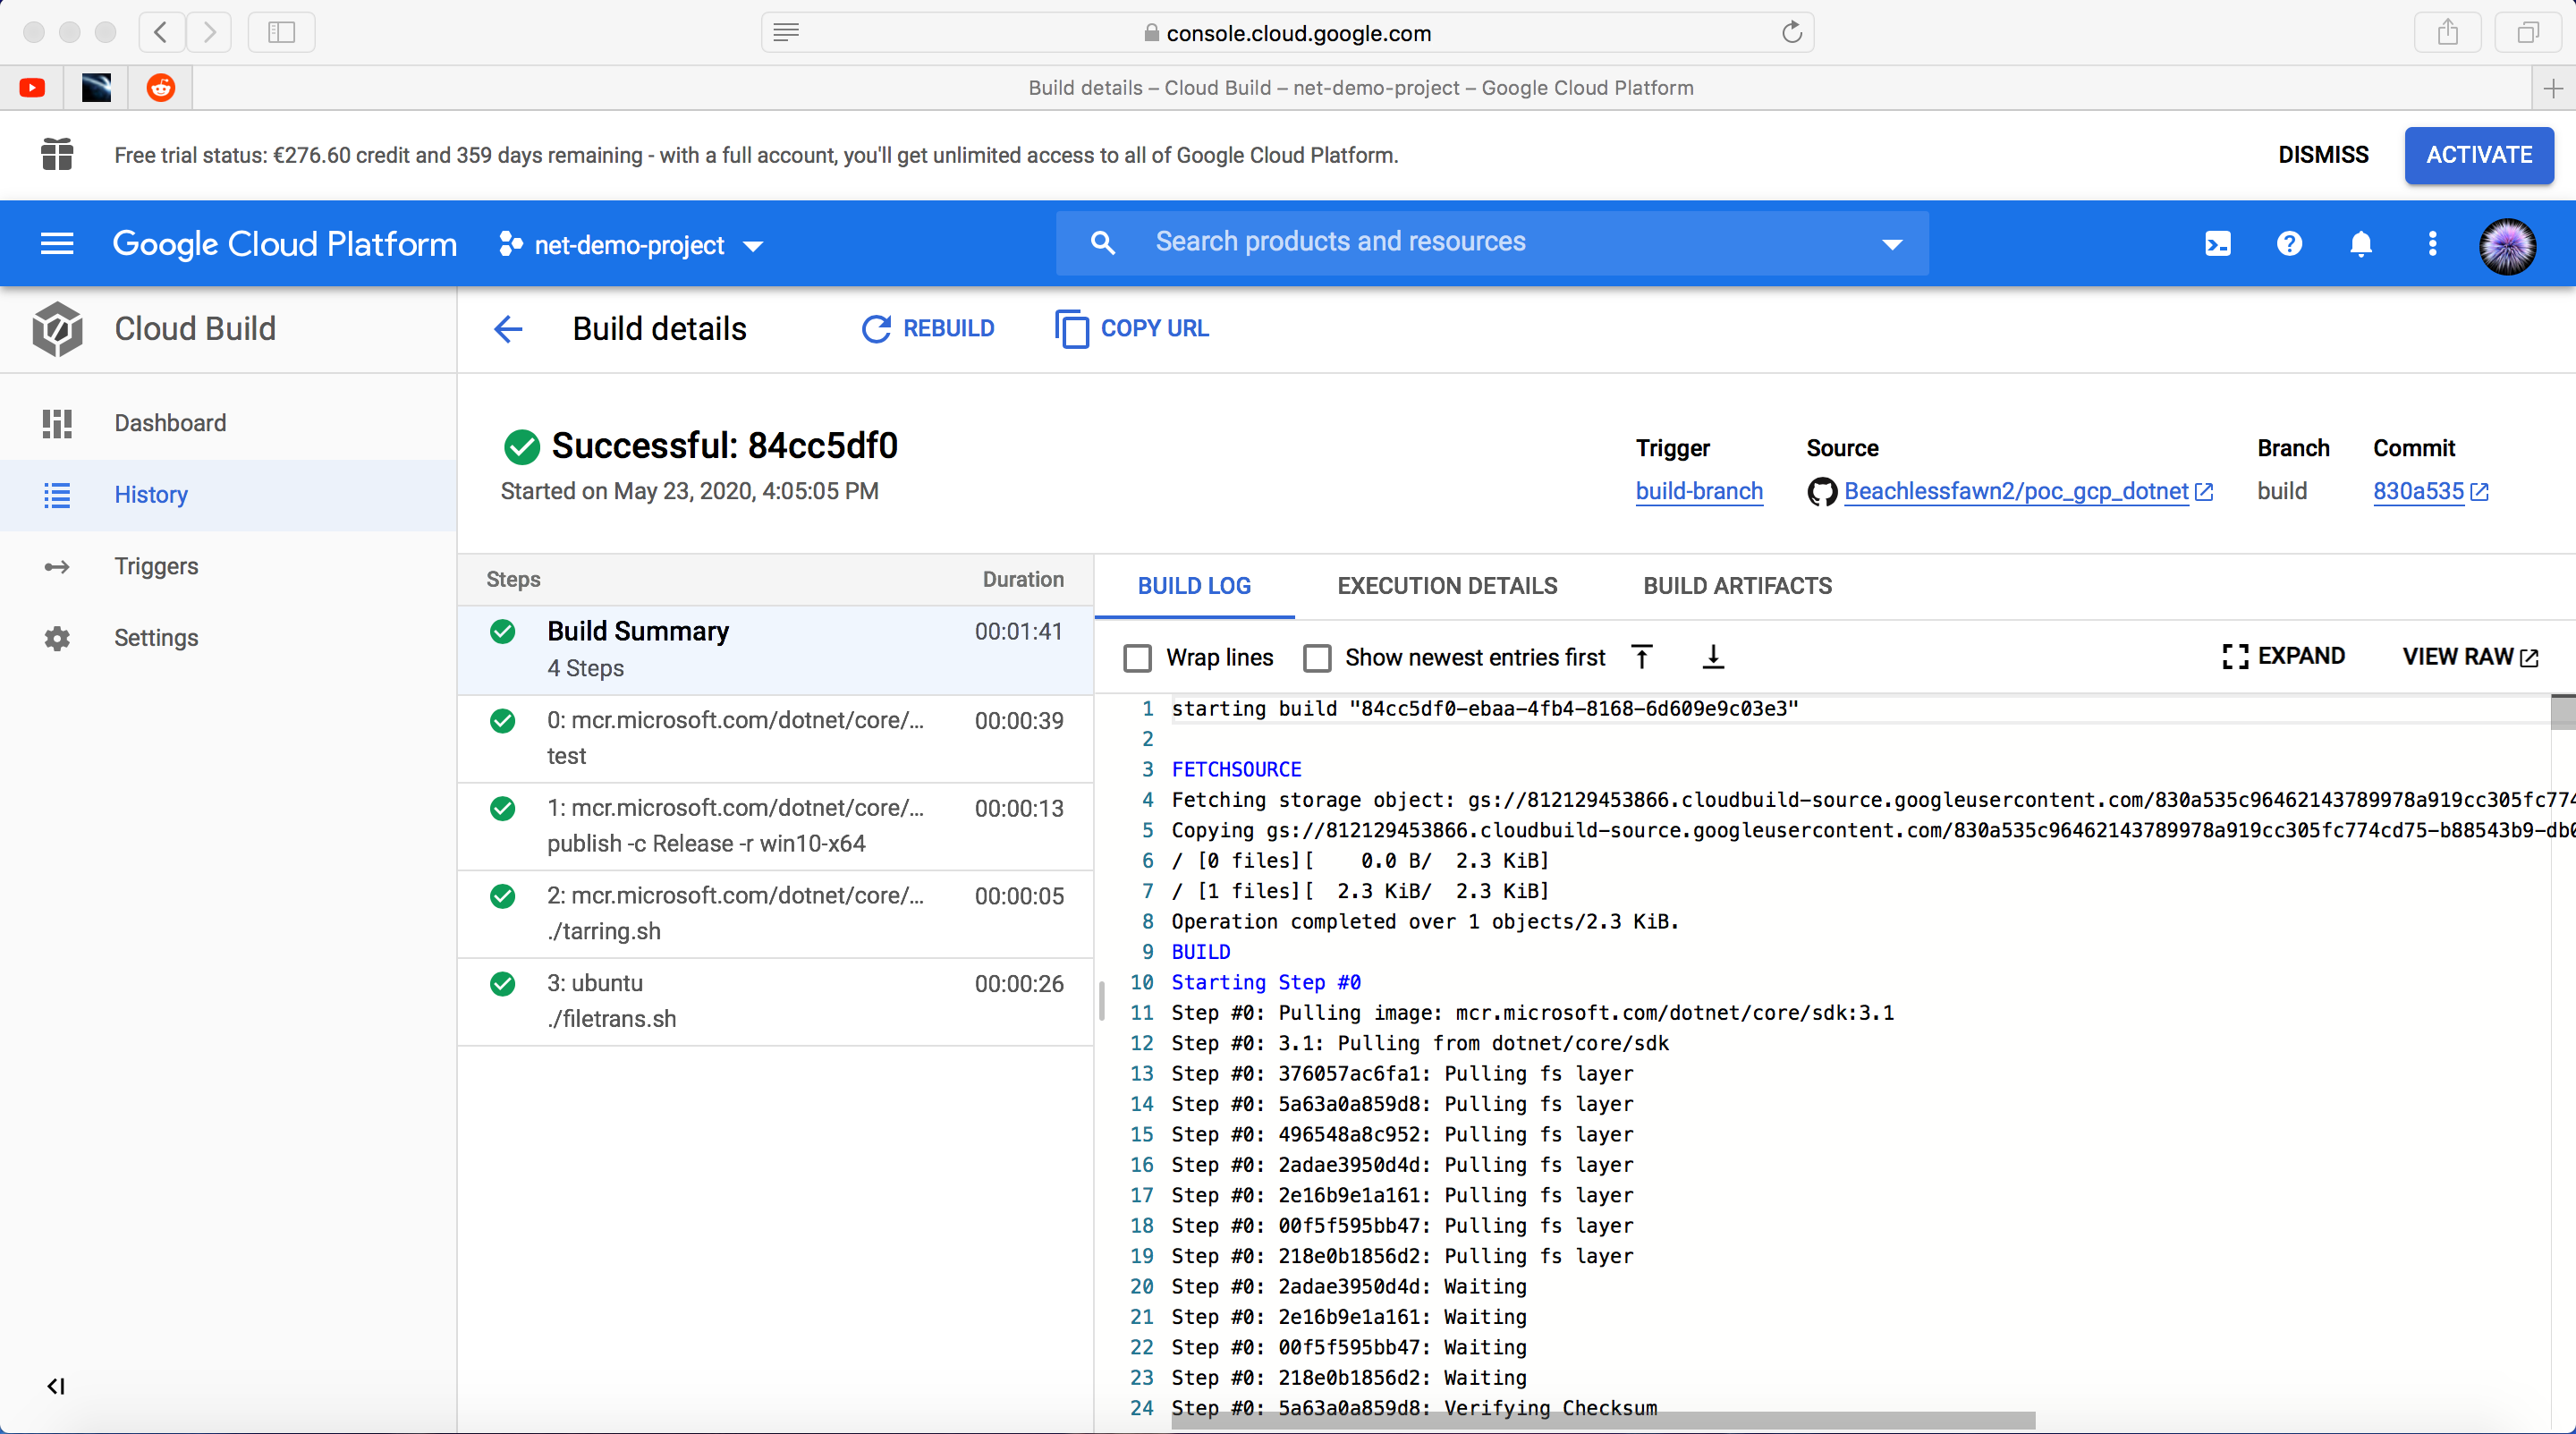
\includegraphics[width=\linewidth]{/Users/kenzie/Documents/HoGent/Bachelorproef/Images/gcp_net_demo_run.png}
    \caption{Console uitvoer van een pipeline op Google Cloud. Figuur toont het resultaat van de compilatie stappen op Google Cloud. Ook zijn er een aantal andere logs te bekijken op dit scherm.}
    \label{fig:GCP_POC_run}
\end{figure}

Tot slot is er op de online console van Google Cloud een simpel dashboard te zien. Dit dashboard toont de laatst uitgevoerde compilatie trigger van het project. Ook toont het eventuele fouten, gemiddelde tijden, wat de compilatie heeft doen uitvoeren, commit ID van GitHub, enz. \emph{Figuur~\ref{fig:GCP_POC_dashboard}} toont een voorbeeld van zo een dashboard.

\begin{figure}[!htbp]
    \centering
    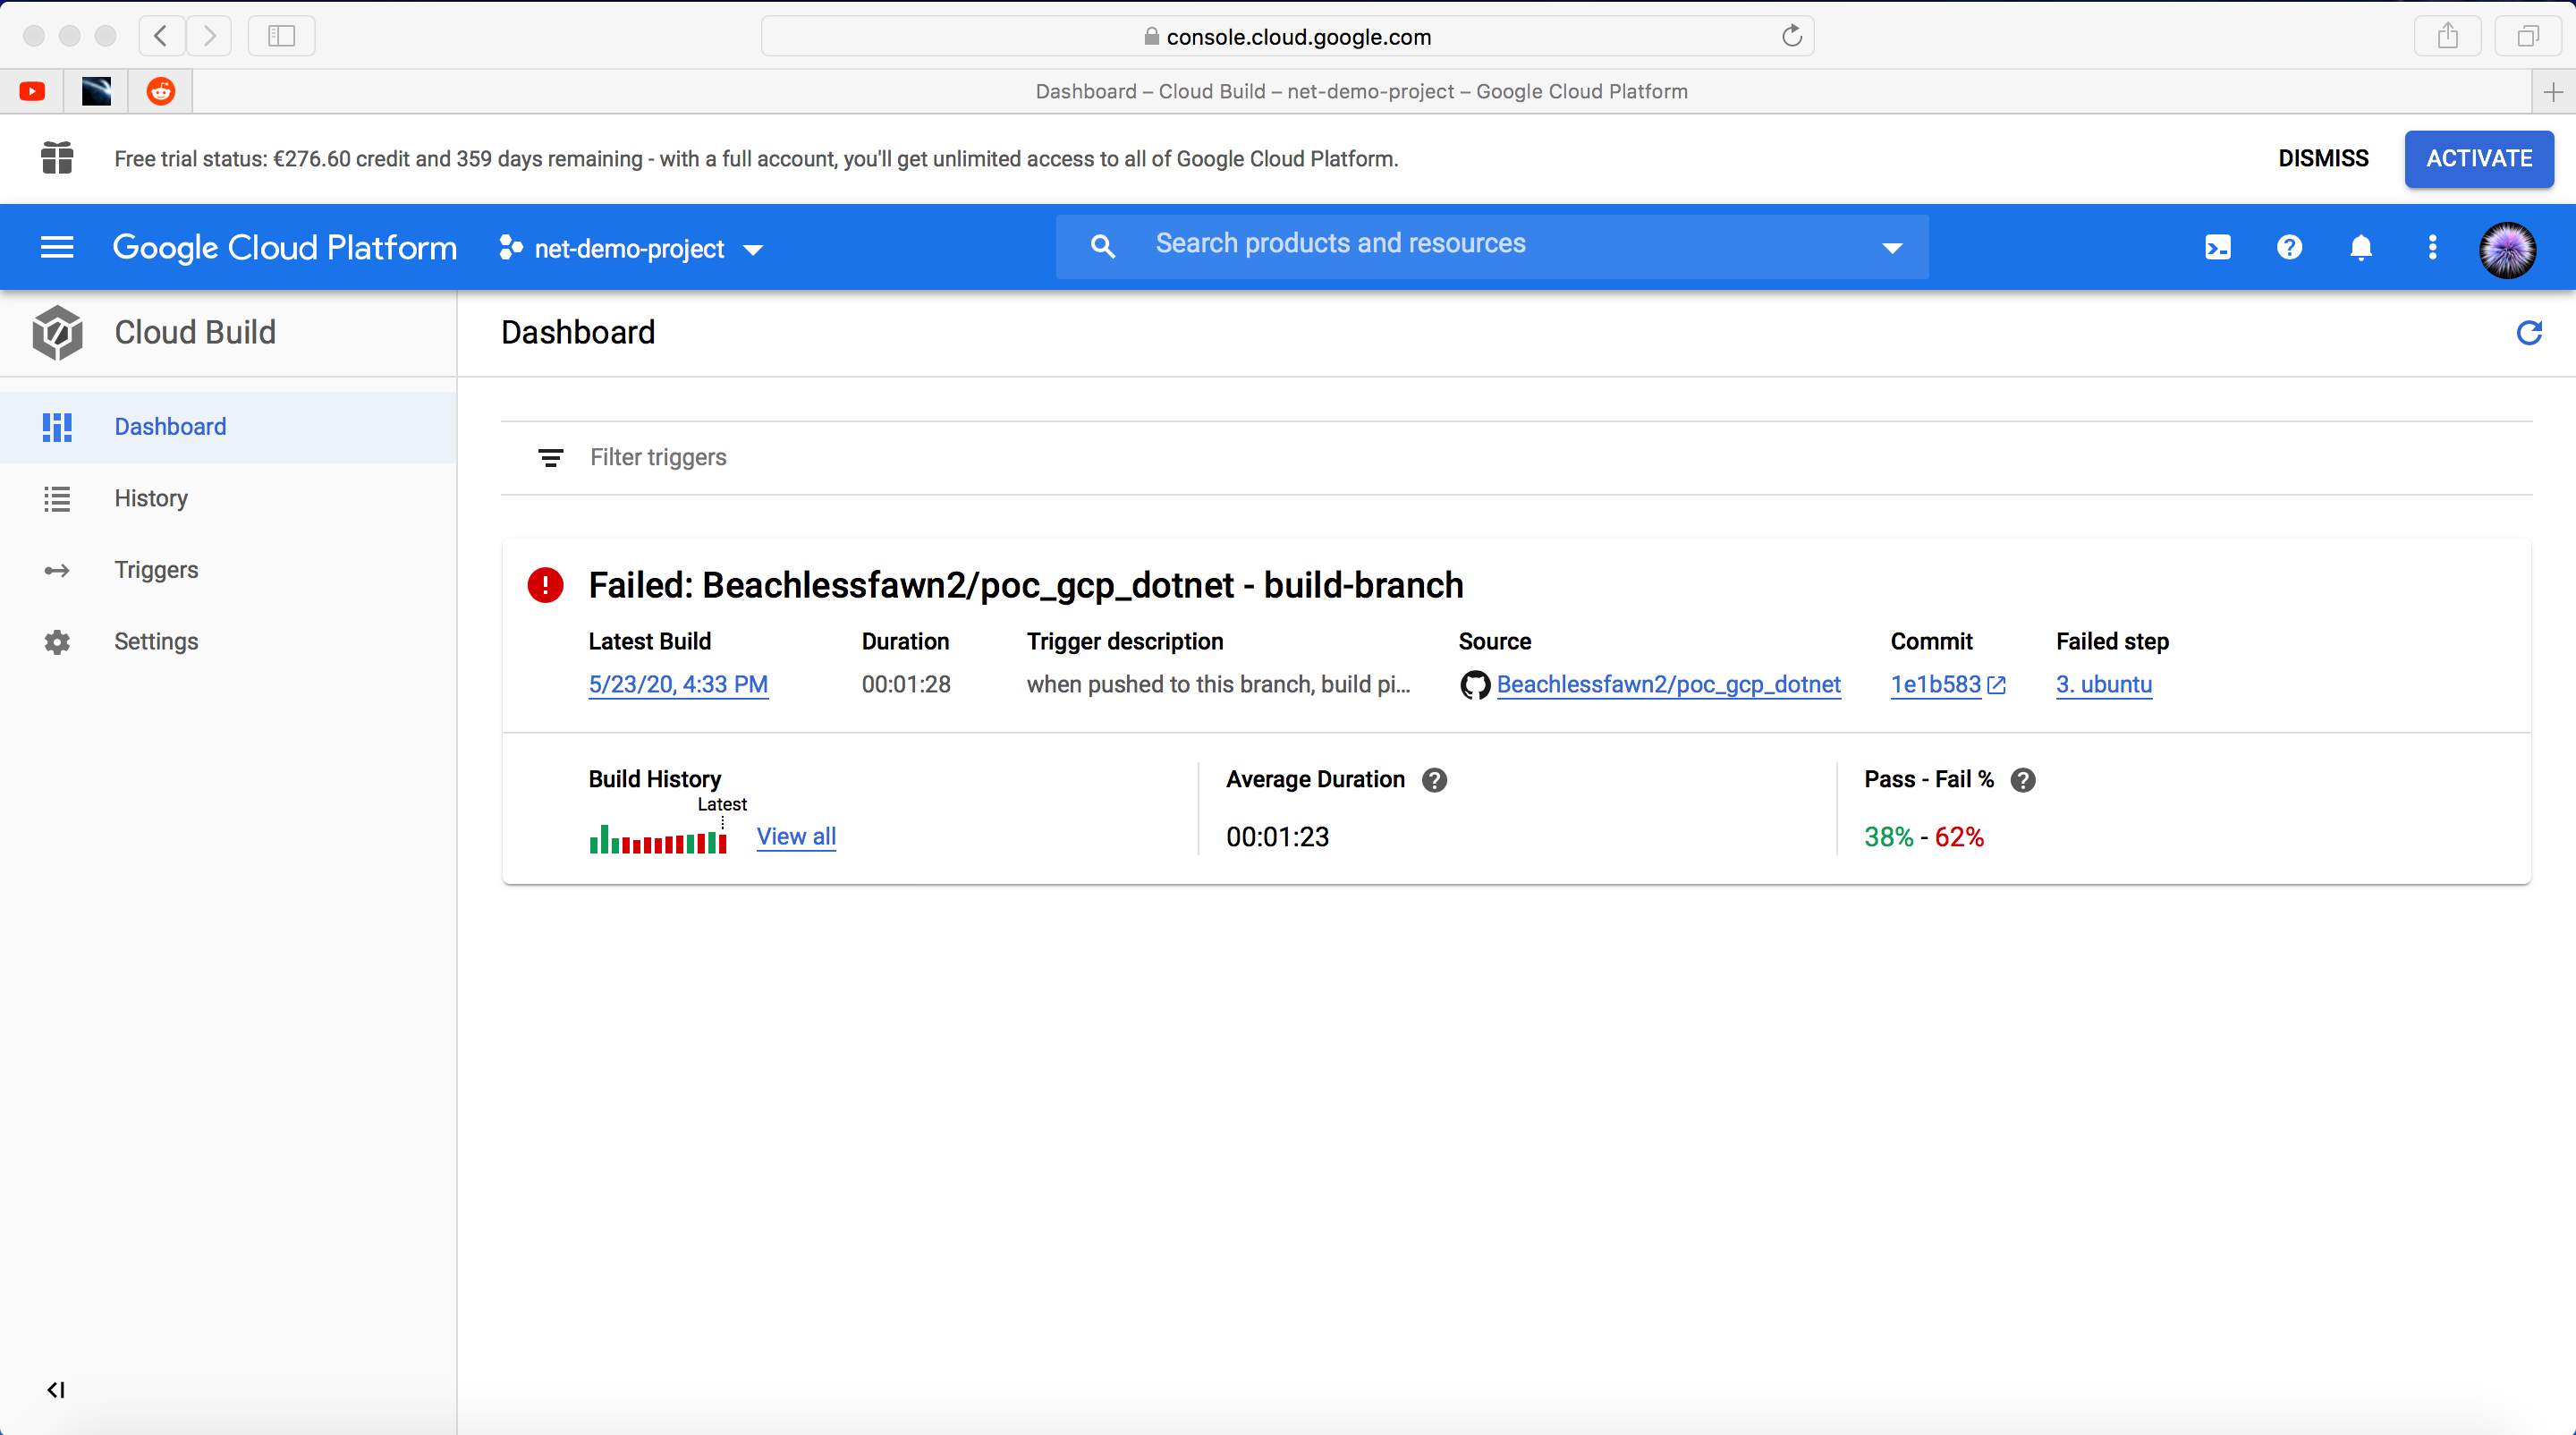
\includegraphics[width=\linewidth]{/Users/kenzie/Documents/HoGent/Bachelorproef/Images/gcp_net_demo_dashboard.png}
    \caption{Compileer resultaten dashboard op Google Cloud. Figuur toont een simpel dashboard met gegevens over de compilatie pipeline.}
    \label{fig:GCP_POC_dashboard}
\end{figure}

Door deze POC op te stellen is er gebleken dat Google Cloud Build Code gemakkelijk te gebruiken is. Dat is, eenmaal de gebruiker er thuis in is. Er bestaat redelijk wat documentatie over wat allemaal mogelijk is in een ‘cloudbuild.yaml’. Helaas is het voor een beginner niet gemakkelijk om te verstaan hoe de verschillende containers met elkaar samenwerken en waar nu alle bestanden staan. Ook is een goede kennis van de containers nodig om te kunnen verstaan wat er allemaal mogelijk is. Dit zorgt ervoor dat het lang kan duren vooraleer er een pipeline operationeel is. Ook is het spijtig dat er niet meer analytics te verkrijgen zijn op Google Cloud Code Build. De gebruiker heeft enkel de analytics van wat er door Google zelf wordt aangeboden. Na het opstellen van deze POC is er ook gebleken dat Google Cloud niet zo duur is. Al het testen en uitproberen heeft slechts 0.40 euro gekost.
Het kan interessant zijn om in een later onderzoek te kijken of het niet mogelijk is om de gegenereerde log bestanden van Google Cloud te downloaden en te gebruiken voor eigen visualisatie systemen zoals: Grafana. 

\subsection{Azure DevOps}
\label{sec:VergelijkingADV}
Naast de POC op Google Cloud is het ook nog interessant om dezelfde opstelling eens te maken in Azure DevOps. Dit om de ervaring en de functionaliteit naast elkaar te kunnen leggen. Voor de POC op Azure DevOps is er een nieuw DevOps project aangemaakt. Dit project heeft de naam ‘poc\_azure\_dotnet’ gekregen. \emph{Figuur~\ref{fig:Azure_POC_proj}} toont het aangemaakte project. Net zoals GCP bevatten projecten alle toegewezen producten en services die zijn geconfigureerd. Ook is het gemakkelijk opnieuw te verwijderen en stopt dan ook de aanrekening.

\begin{figure}[!htbp]
    \centering
    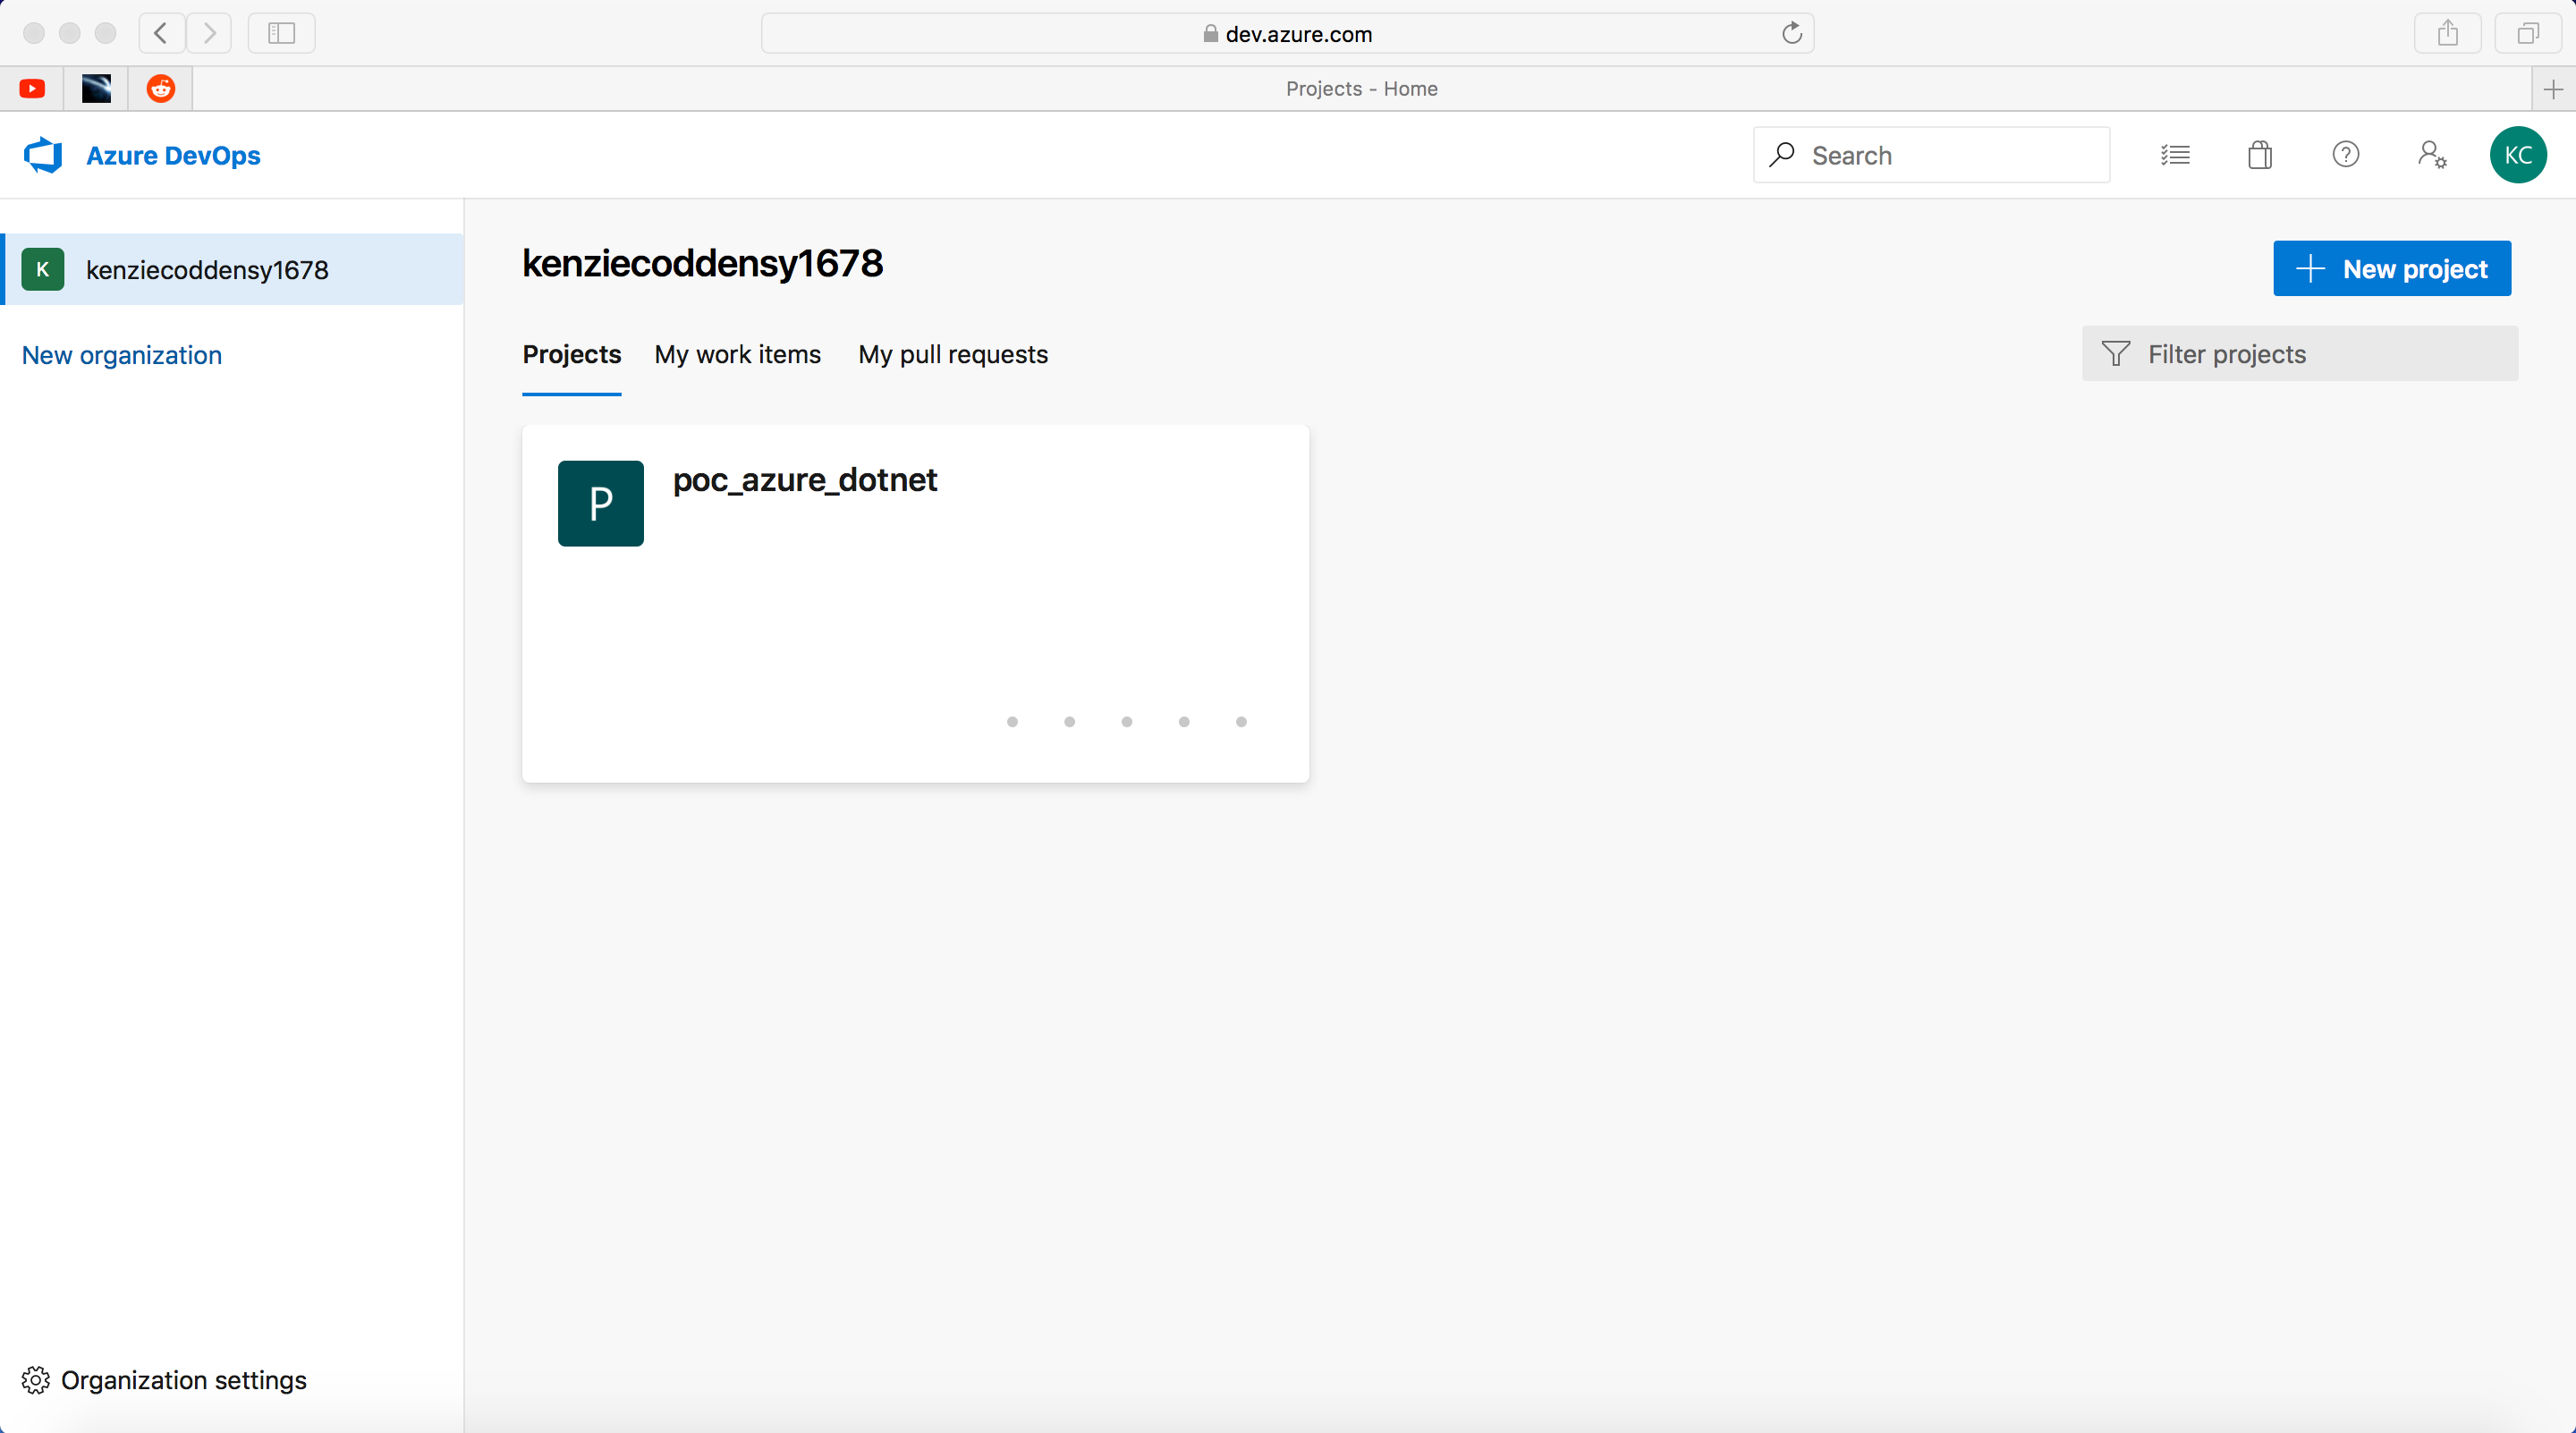
\includegraphics[width=\linewidth]{/Users/kenzie/Documents/HoGent/Bachelorproef/Images/azure_net_demo_proj.png}
    \caption{Hoofd scherm Azure DevOps. Figuur toont een nieuw aangemaakt project op Azure DevOps.}
    \label{fig:Azure_POC_proj}
\end{figure}

Deze POC vertrekt vanuit dezelfde applicatie als bij GCP. Hiervoor is er een nieuwe map aangemaakt op de gebruiker zijn computer voor de applicatie. Deze is geïnitialiseerd als een Git repository. Hierin zijn dan de bestanden \emph{MessageUtil~\ref{code:messageutil}} \& \emph{MessageUtilTest~\ref{code:messageutiltest}} voor de .Net applicatie in geplaatst. Ook is er een gitignore aangemaakt. \emph{Figuur~\ref{code:azuregittree}} toont een tree van de bestanden en mappen structuur. Deze repository is dan geüpload naar GitHub.

\lstset{
    language=bash,
    caption={Tree van de bestanden structuur voor de Proof Of Concept op Azure DevOps.},
    label=code:azuregittree
}
\begin{lstlisting}
poc_azure_dotnet/
`--- .gitignore
`--- MessageUtil
`--- MessageUtil.csproj
`--- MessageUtilProgram.cs
`--- MessageUtil.sln
`--- MessageUtilTest
`--- MessageUtilTest.csproj
`--- MessageUtilTests.cs
\end{lstlisting}

Hierna is er op Azure DevOps een nieuwe pijpleiding aangemaakt. Dit was zeer gemakkelijk te volgen door middel van de online wizard. Eerst moest er gekozen worden wat versiebeheersysteem de gebruiker gebruikt. Hier is er gekozen voor GitHub. Vervolgens vraagt Azure DevOps de gebruiker toestemming voor het uitlezen van de repositories. Tegelijk wordt ook de Azure DevOps applicatie toegevoegd aan de gebruiker zijn GitHub. Na de initialisatie van de Azure DevOps applicatie voor GitHub moest er een reposirotry worden geselecteerd. Hier is er gekozen voor de zojuist gemaakte GitHub repository. Azure DevOps leest deze repository uit en stelt dan op basis van de bestanden de juiste compilatie oplossing voor. Voor deze POC stelde Azure DevOps .Net Core voor als compilatie programma. Er is voor dezen oplossing gekozen. Azure DevOps toont hierna een Yaml-bestand, ‘azure-pipelines.yml’, met voor gemaakte stappen. Dit YAML-bestand bevat drie stappen. Een eerste stap die de juiste pakketten installeert op de virtuele machine. In een tweede stap wordt de applicatie gecompileerd. In de derde stap worden de meegeleverde testen uit \emph{MessagUtilTest~\ref{code:messageutiltest}} uitgevoerd. \emph{Figuur~\ref{code:azure-pipelines-poc}} toont dit YAML-bestand.

\lstset{
    language=bash,
    caption={YAML-bestand voor de configuratie van de .Net pipeline op Azure DevOps.},
    label=code:azure-pipelines-poc
}
\begin{lstlisting}
# .NET Desktop
# Build and run tests for .NET Desktop or Windows classic desktop solutions.
# Add steps that publish symbols, save build artifacts, and more:
# https://docs.microsoft.com/azure/devops/pipelines/apps/windows/dot-net

trigger:
- master

pool:
vmImage: 'windows-latest'

variables:
solution: '**/*.sln'
buildPlatform: 'Any CPU'
buildConfiguration: 'Release'

steps:
- task: NuGetToolInstaller@1

- task: NuGetCommand@2
inputs:
restoreSolution: '$(solution)'

- task: VSBuild@1
inputs:
solution: '$(solution)'
platform: '$(buildPlatform)'
configuration: '$(buildConfiguration)'

- task: VSTest@2
inputs:
platform: '$(buildPlatform)'
configuration: '$(buildConfiguration)'
\end{lstlisting}

Verwacht was dat dit een werkend vertrekpunt is voor de pipeline. Zeker omdat deze applicatie met een Microsoft specifieke taal is gemaakt, met behulp van het .Net framework dat ook Microsoft specifiek is. In eerste instantie leek deze pipeline te werken. Maar na het bekijken van de logbestanden is er vastgesteld dat de testen niet werden uitgevoerd. Er is gezocht naar een oplossing voor dit probleem. Er is geen duidelijke oplossing gevonden voor de huidige configuratie. De documentatie over deze modules was zeer onduidelijk en moeilijk te begrijpen. Zeker vanuit het standpunt van een beginner. In dit opzicht is er gekozen om opnieuw te beginnen aan de hand van een andere \emph{\href{https://docs.microsoft.com/en-us/azure/devops/pipelines/ecosystems/dotnet-core?view=azure-devops}{handleiding}} op Azure. Deze gebruikt een voor gemaakte Windows virtuele machine met .Net core geïnstalleerd. Over deze module is uitgebreide documentatie te vinden. Daarnaast zijn er door Microsoft ook voorbeelden ter beschikking. Dit was dan ook het perfecte vertrekpunt.

Dit nieuw YAML-bestand bestaat uit zes stappen. In een eerste stap wordt de ‘MessageUtil’ applicatie volledige herbouwt. Deze staat dan klaar voor verdere stappen. In de tweede stap wordt de applicatie gecompileerd. De derde stap voert de meegeleverde testen uit. Ook publiceert het de resultaten op Azure DevOps. \emph{Figuur~\ref{fig:Azure_POC_testr}} toont een voorbeeld van uitgevoerde testen. De vierde stap compileert een uitrol versie voor het '64 bit Windows 10' platform in een map, publish. In de vijfde stap wordt er een PowerShell script uitgevoerd. Dit Script comprimeert de map publish. \emph{Figuur~\ref{code:zipping}} toont het ‘zipping.ps1’ script. In een laatste stap wordt deze gecomprimeerde map gepubliceerd als een artifact zodanig dat de applicatie klaarstaat om in een latere stap te worden uitgerold. \emph{Figuur~\ref{code:azure-pipelines-poc-n}} toont het verbeterde ‘azure-pipelines.yml’. Vervolgens is deze code toegevoegd op GitHub.

\begin{figure}[!htbp]
    \centering
    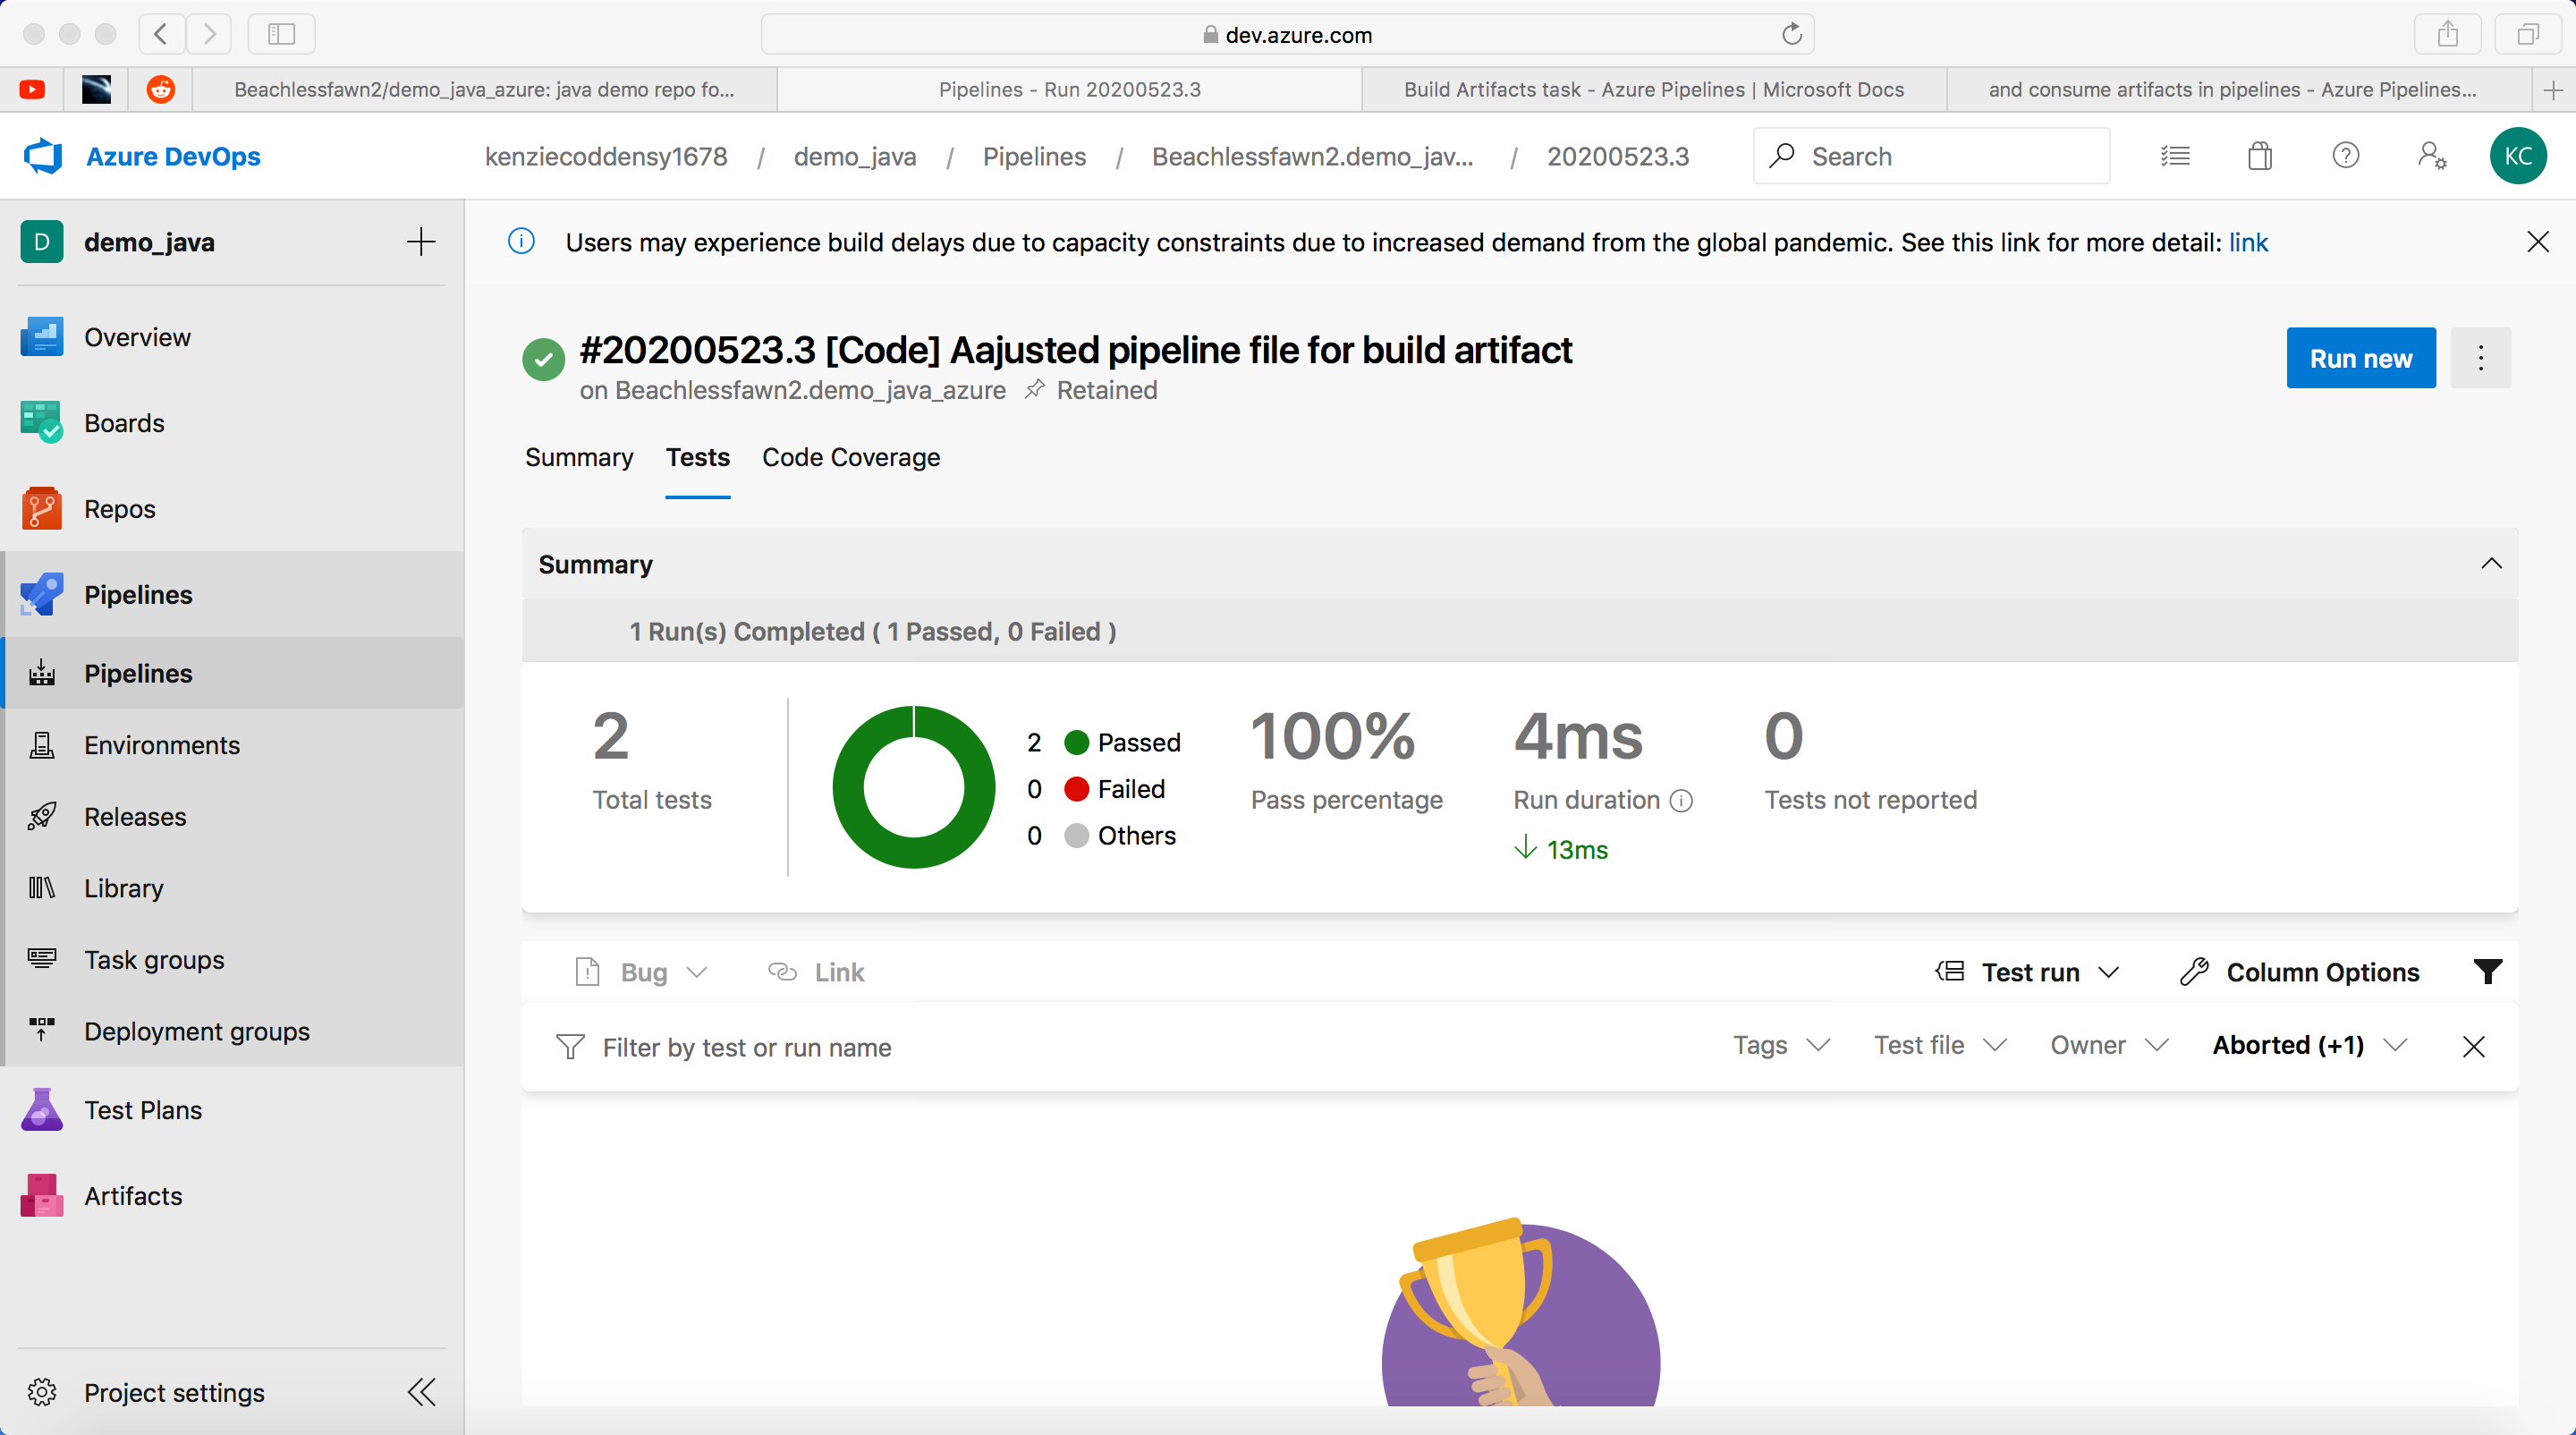
\includegraphics[width=\linewidth]{/Users/kenzie/Documents/HoGent/Bachelorproef/Images/azure_net_demo_testr.png}
    \caption{Test-pass dashboard Azure DevOps. Figuur toont een simpel dashboard met gegevens over de uitgevoerde testen.}
    \label{fig:Azure_POC_testr}
\end{figure}

\lstset{
    language=C,
    caption={PowerShell script dat een map compresseert. Wordt gebruikt om alle .Net Framework afhankelijkheden mee te verpakken.},
    label=code:zipping
}
\begin{lstlisting}
$compress = @{
Path= "d:\a\1\s\MessageUtil\bin\Release\netcoreapp3.1\win10-x64\publish\*"
CompressionLevel = "Fastest"
DestinationPath = "d:\a\1\s\MessageUtil.zip"
}
Compress-Archive @compress
\end{lstlisting}

\lstset{
    language=bash,
    caption={Verbeterd YAML-bestand voor de configuratie van de .Net pipeline op Azure DevOps.},
    label=code:azure-pipelines-poc-n
}
\begin{lstlisting}
trigger:
- master

pool:
vmImage: 'windows-latest'

variables:
buildConfiguration: 'Release'
runtimeIdentifier: 'win10-x64'

steps:
- task: DotNetCoreCLI@2
inputs:
command: 'restore'
restoreDirectory: '$(System.DefaultWorkingDirectory)'
#packDirectory: '$(System.DefaultWorkingDirectory)'
displayName: 'DotNet Restore Project'

- task: DotNetCoreCLI@2
inputs:
command: 'build'
arguments: '--configuration $(buildConfiguration)'
displayName: 'DotNet Build $(buildConfiguration)'

- task: DotNetCoreCLI@2
inputs:
command: 'test'
projects: '**/*Test/*.csproj'
arguments: '--configuration $(buildConfiguration) --collect "Code coverage"'
displayName: 'DotNet Test Build'

- task: DotNetCoreCLI@2
inputs:
command: 'publish'
publishWebProjects: false
arguments: '--configuration $(buildConfiguration) -r $(runtimeIdentifier)'
zipAfterPublish: false
displayName: 'DotNet Publish Build'

- task: PowerShell@2
inputs:
targetType: 'filePath'
filePath: $(System.DefaultWorkingDirectory)\ziping.ps1
errorActionPreference: 'stop'
displayName: 'DotNet Zip Publish'

- task: PublishPipelineArtifact@1
inputs:
targetPath: $(System.DefaultWorkingDirectory)\MessageUtil.zip
artifactName: MessageUtil
displayName: 'Upload Zip'
\end{lstlisting}

Het CI-gedeelte van de pipeline werkt met deze code. Voor het CD-gedeelte moest er een nieuwe release pipeline worden gemaakt. Op Azure DevOps is er een nieuwe release gemaakt bestaande uit een Linux Ubuntu machine. Deze virtuele machine download het gemaakte artifact en verzend dit bestand naar de lokale Windows Server. Deze virtuele machine voert het script uit \emph{figuur~\ref{code:filetrans}} uit. Het instellen van deze release pipeline is zeer gemakkelijk door de online wizard. \emph{Figuur~\ref{fig:Azure_POC_release}} toont het instellen van de virtuele machine. Ook zijn er talloze opties voor het instellen van toestemmingen, rechten, controles, enz. Dit kan interessant zijn in een productie omgeving. Deze POC laat dit buiten beschouwing. \emph{Figuur~\ref{fig:Azure_POC_pijp}} toont de volledige pipeline.

\begin{figure}[!htbp]
    \centering
    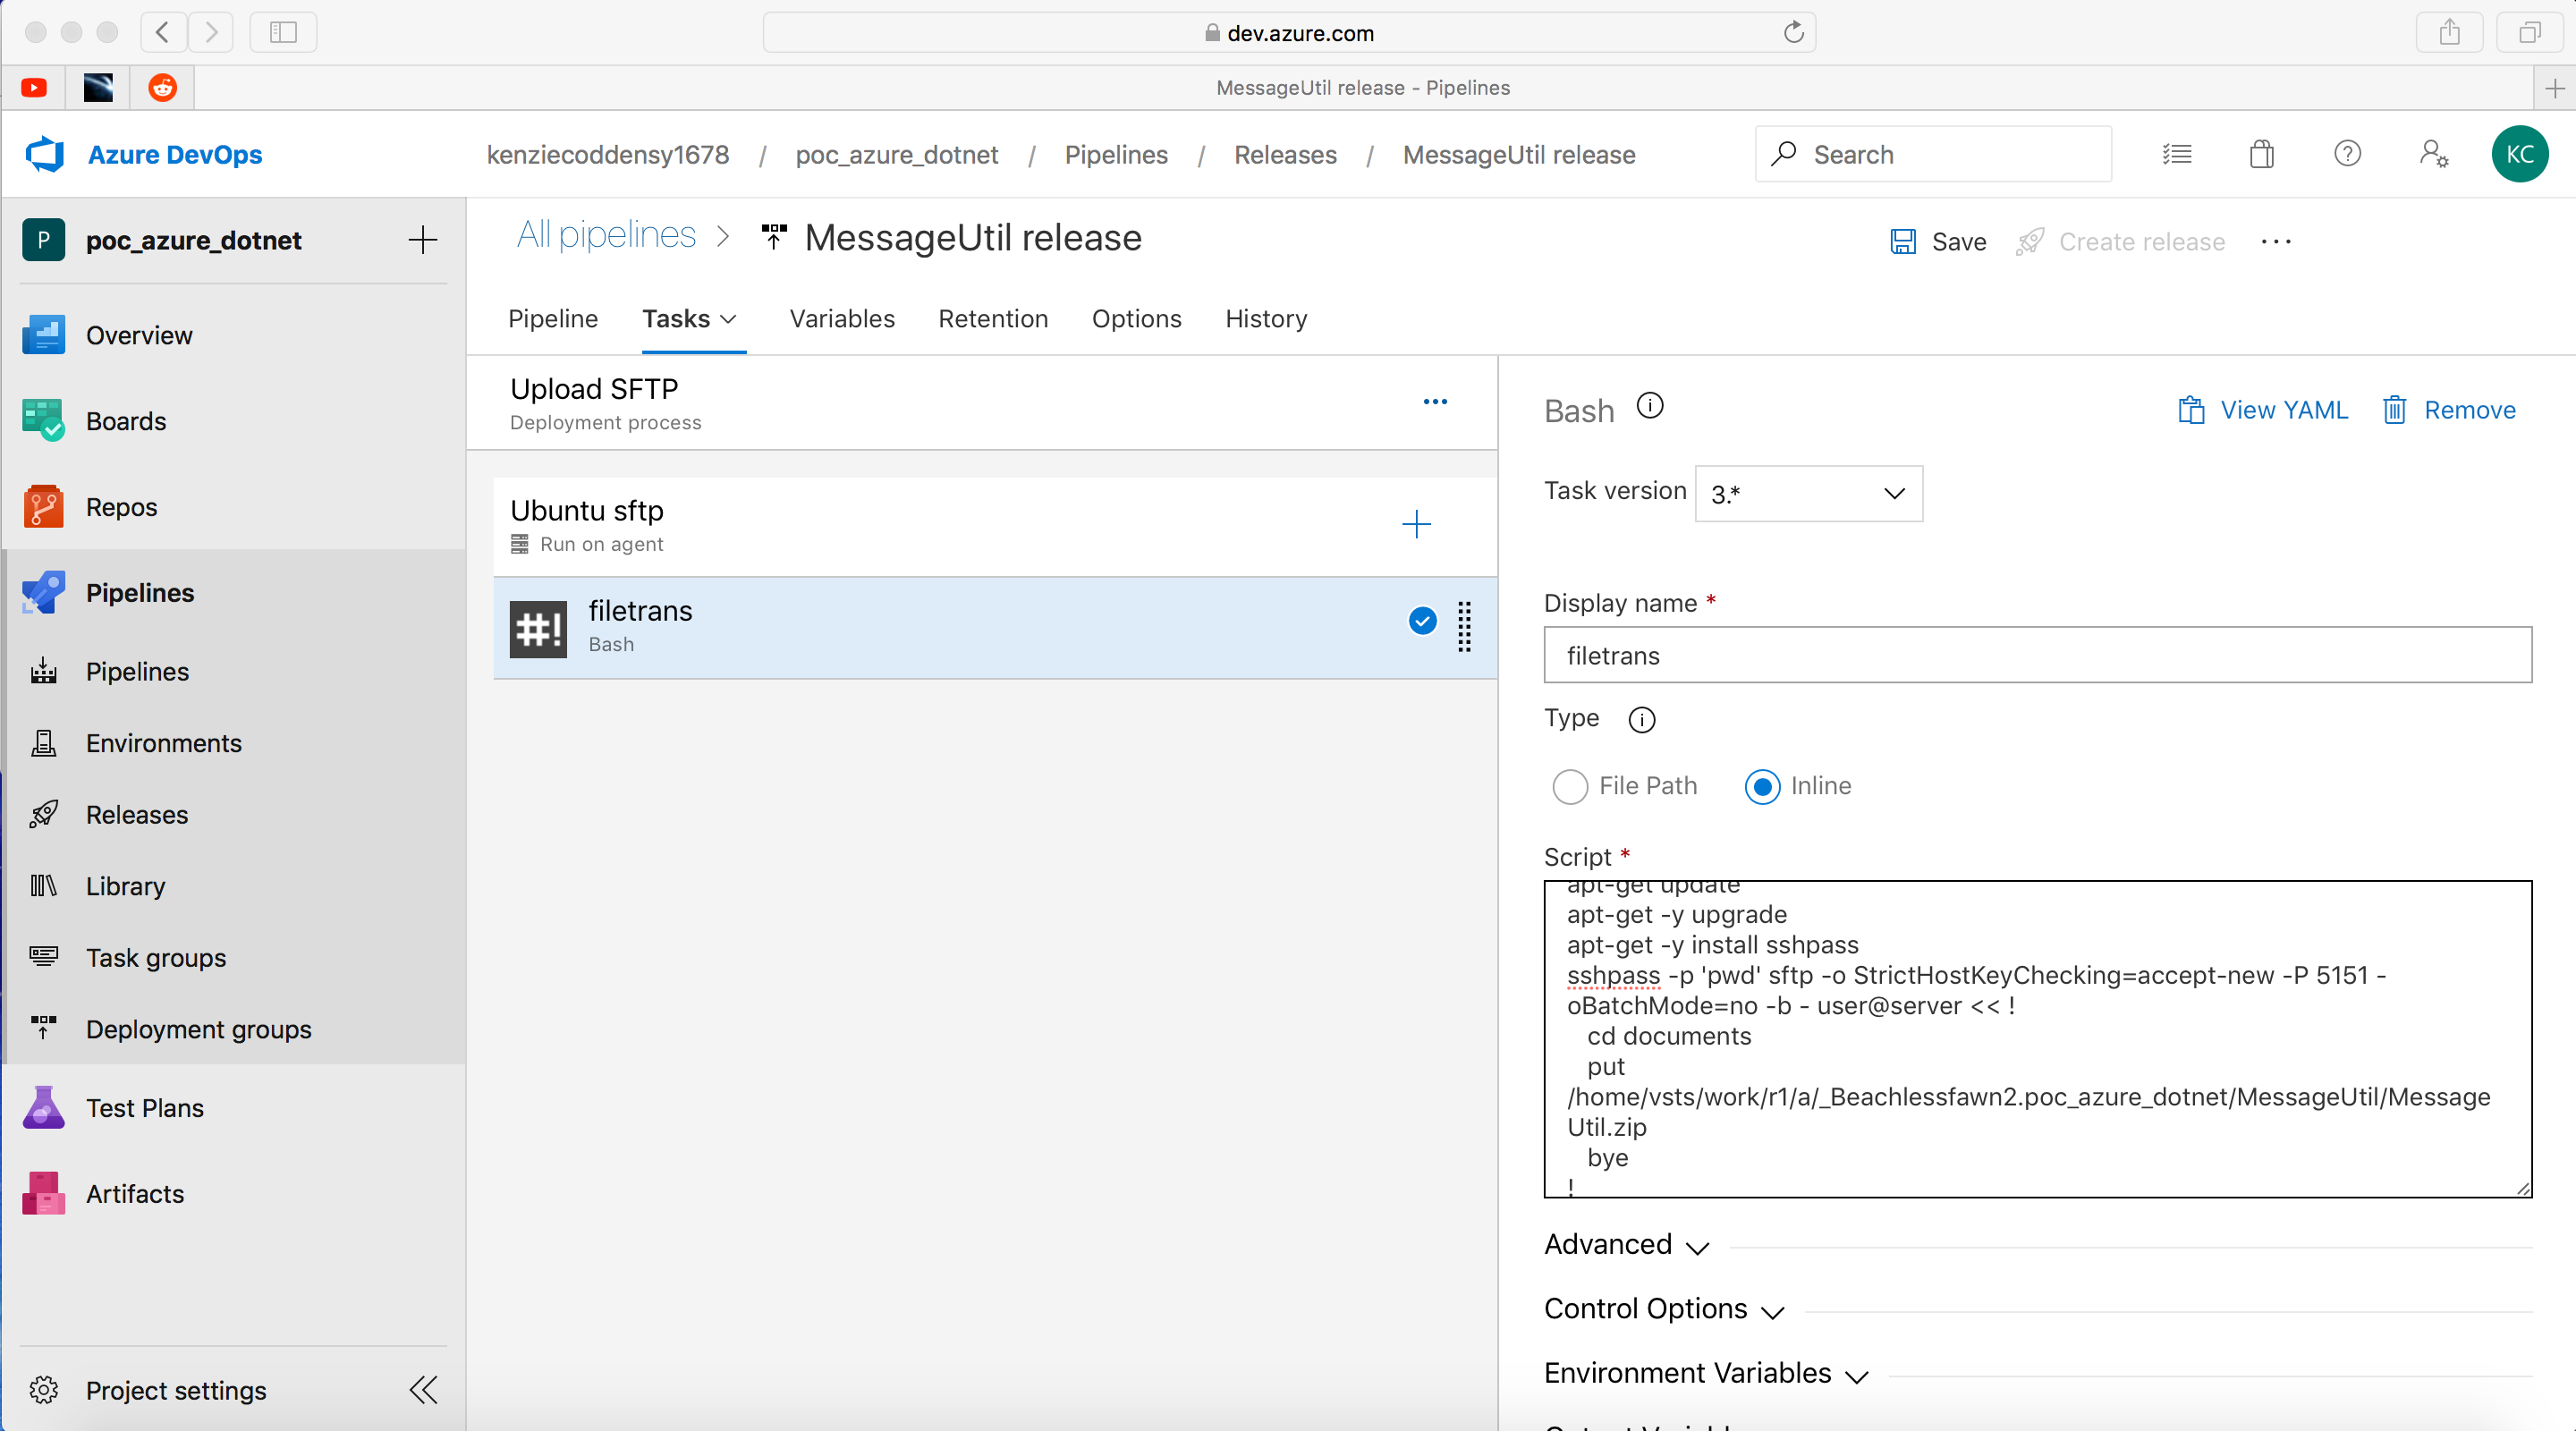
\includegraphics[width=\linewidth]{/Users/kenzie/Documents/HoGent/Bachelorproef/Images/azure_net_demo_release.png}
    \caption{Release pipeline configuratie. Figuur toont hoe een release pipeline op Azure DevOps wordt geconfigureerd. In dit geval wordt er een Ubuntu machine geconfigureerd met een script.}
    \label{fig:Azure_POC_release}
\end{figure}

\begin{figure}[!htbp]
    \centering
    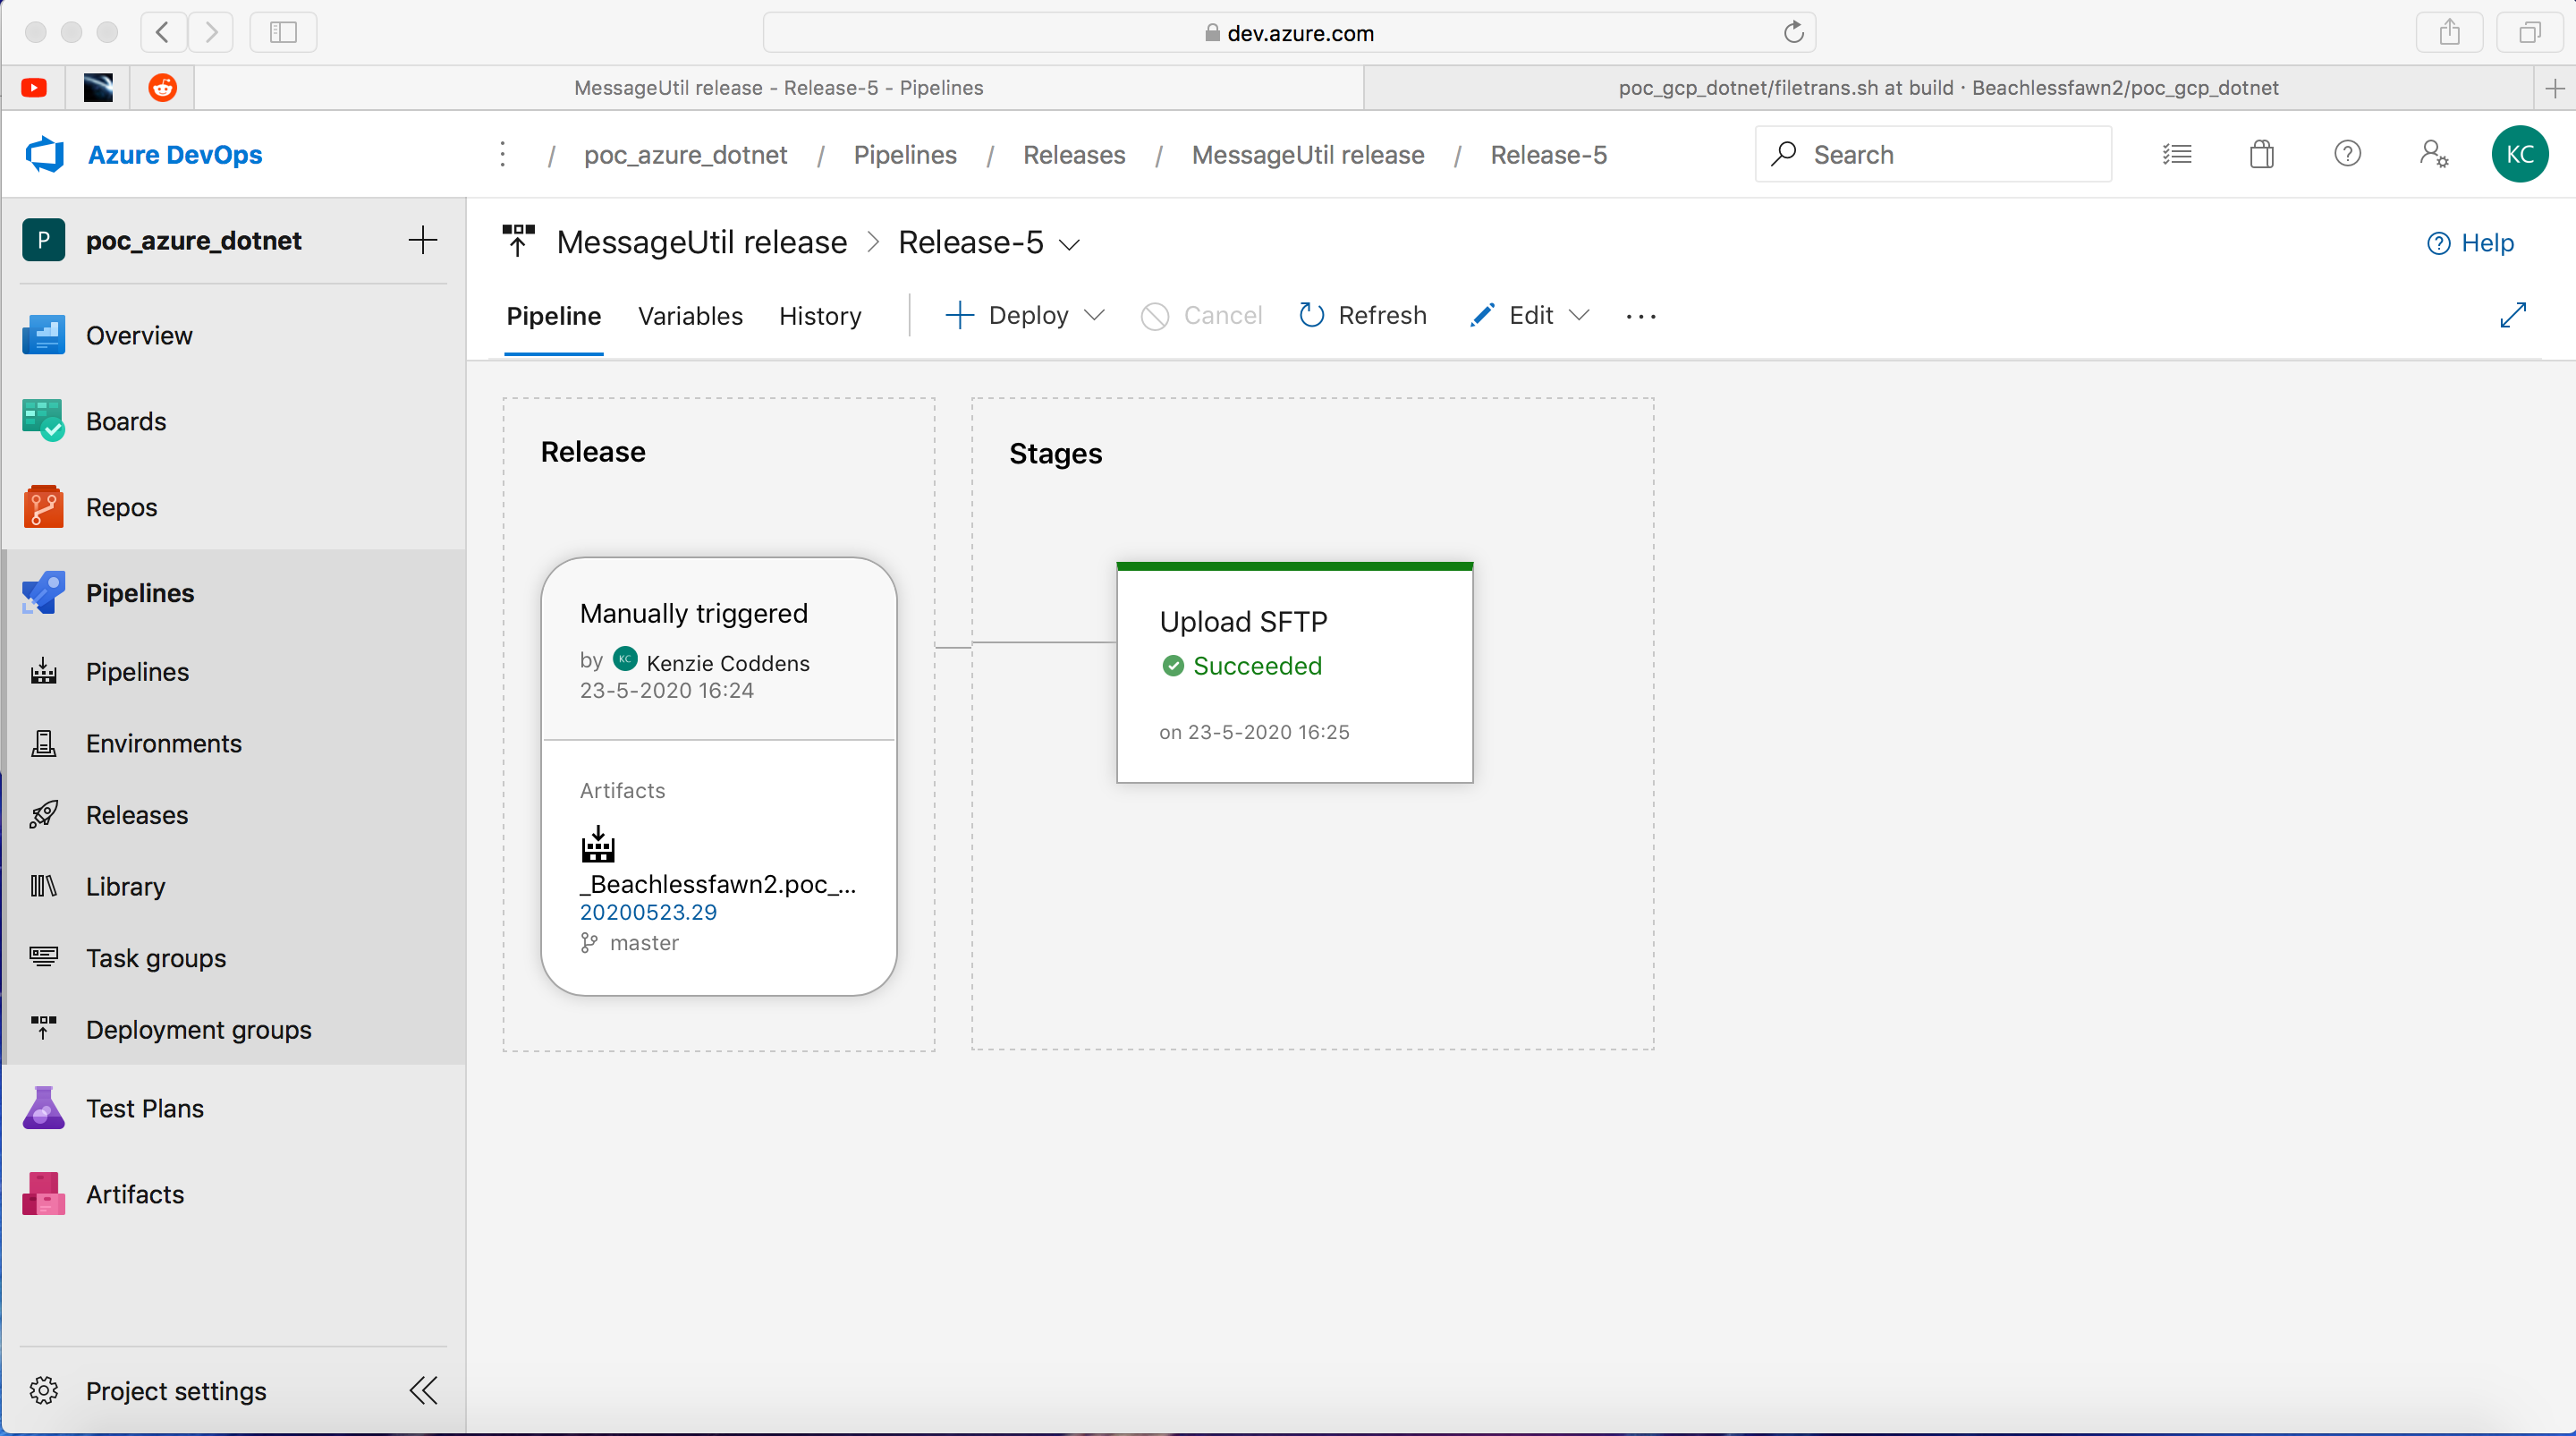
\includegraphics[width=\linewidth]{/Users/kenzie/Documents/HoGent/Bachelorproef/Images/azure_net_demo_pijp.png}
    \caption{Grafische weergave Azure DevOps pipeline. De figuur toont een kort overzicht van de totale pipeline op Azure DevOps.}
    \label{fig:Azure_POC_pijp}
\end{figure}

Azure DevOps heeft ook zeer goede analytics. Voor deze POC zijn er een aantal voorbeelden gemaakt. Net zoal Google Cloud heeft Azure ook Dashboards. \emph{Figuur~\ref{fig:Azure_POC_dashboard}} toont een overzicht van het project.

\begin{figure}[!htbp]
    \centering
    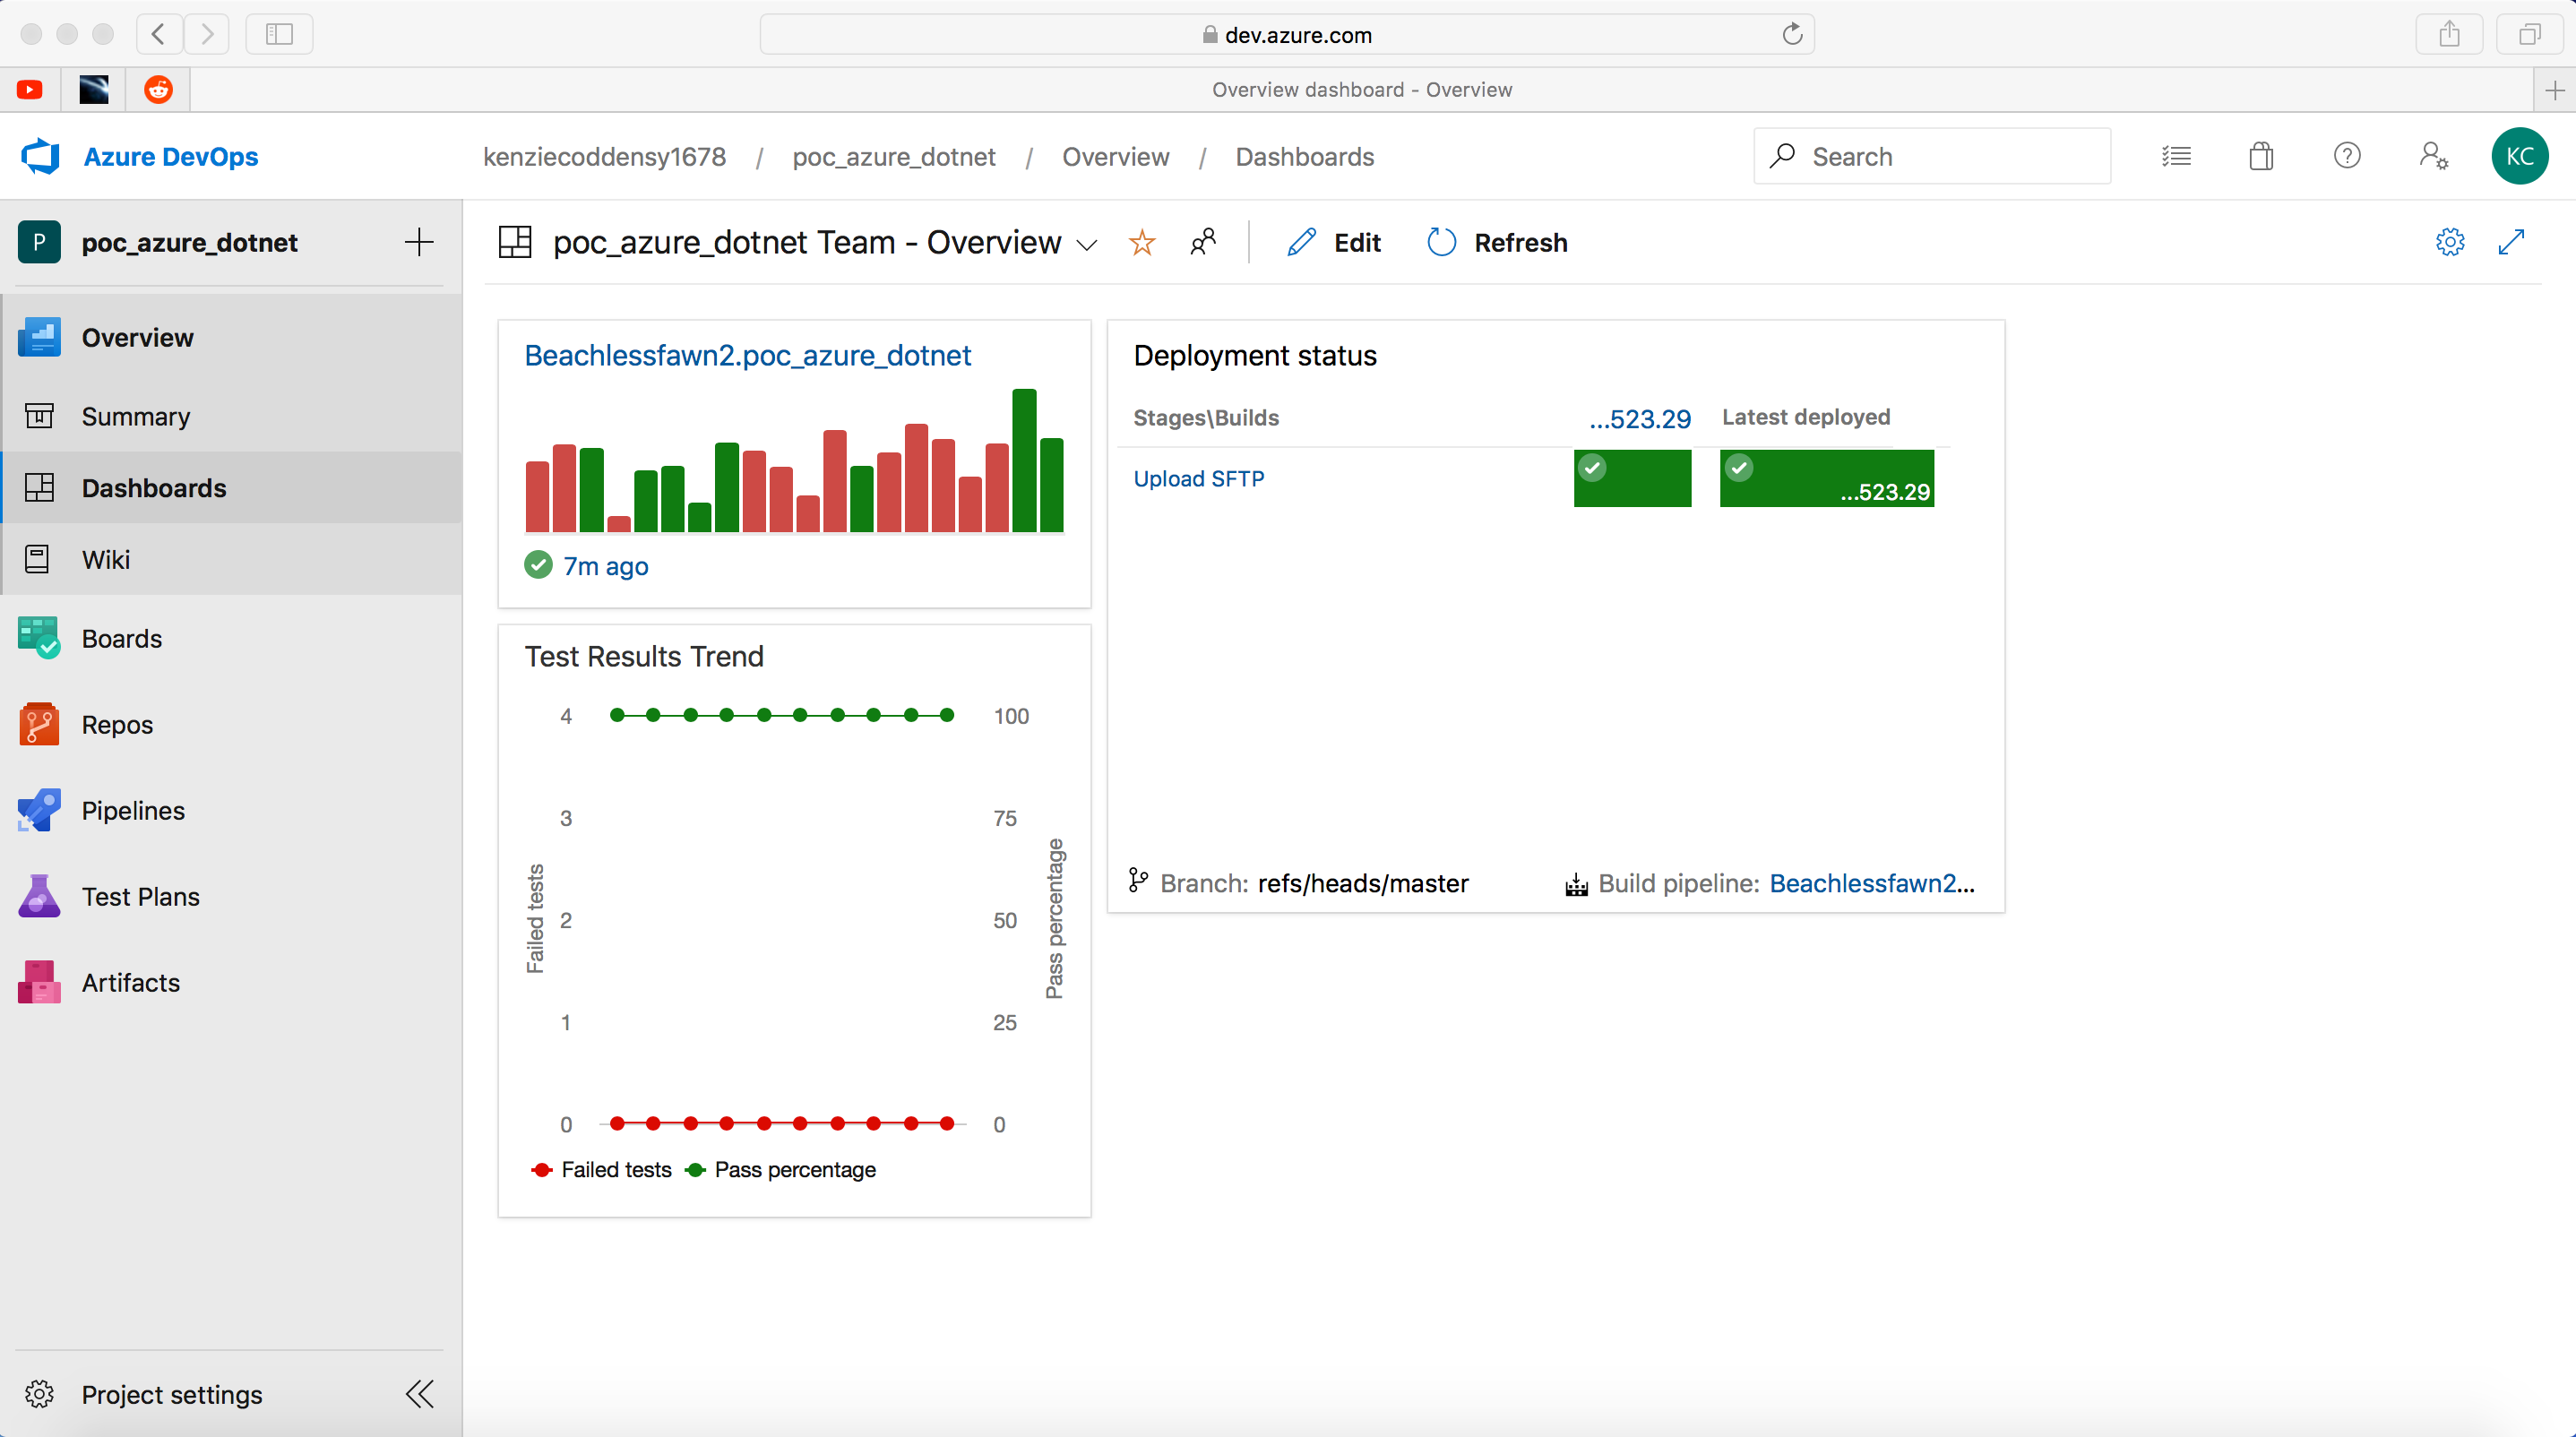
\includegraphics[width=\linewidth]{/Users/kenzie/Documents/HoGent/Bachelorproef/Images/azure_net_demo_dashboard.png}
    \caption{Project overzicht dashboard Azure DevOps. Figuur toont een simpel dashboard met gegevens over de compilatie pipeline.}
    \label{fig:Azure_POC_dashboard}
\end{figure}

Uit deze POC is gebleken dat Azure DevOps veel minder complex is om te configureren dan Google Cloud Code Build. Dit komt door de gemakkelijk te gebruiken wizards die de gebruiker door de configuratie heen gidsen. Zo voelt de complexiteit van het configureren van een pipeline minder zwaar aan. Uit deze POC is gebleken dat de standaardoplossing die Azure DevOps voorstelt niet altijd even gemakkelijk is om aan te passen naar de gebruiker zijn noden. Deze POC heeft ook aangetoond dat de documentatie van Azure DevOps complex kan zijn. Zelfs na meerdere projecten te hebben getest, zijn sommige zaken nog niet helemaal duidelijk. Azure DevOps biedt zeer uitgebreide hulpmiddelen aan om allerlei data te visualiseren. Deze dashboards zijn gemakkelijk te creëren. Ook zijn deze duidelijk en overzichtelijk. Dit in tegenstelling tot Google Cloud. In vergelijking met Azure DevOps is Google Cloud gemakkelijker om aangepaste pipelines te maken. Dit omdat het intuïtiever is om de configuratie YAML-bestanden te maken. Ook omdat Google Cloud Code Build met Docker containers werkt. Dit zorgt ervoor dat compileer machines veel uitgebreider kunnen worden aangepast naar de noden van de gebruiker.

Benaderd vanuit het Microsoft ecosysteem is Azure DevOps een zeer goede en logische keuze. Zeker omdat een hele hoop producten en services, die anders aanvullende kosten hebben, vrij te gebruiken zijn. Ook zijn alle hulpmiddelen om software te ontwikkelen volledig geïntegreerd in het platform. Gebruikers die buiten dit ecosysteem werken kijken beter naar Google Cloud in samenwerking met andere hulpmiddelen en oplossingen.